\documentclass{article}

\PassOptionsToPackage{numbers, compress}{natbib}
\usepackage[main, final]{neurips_2026}
\usepackage[utf8]{inputenc}
\usepackage[T1]{fontenc}
\usepackage{hyperref}
\usepackage{url}
\usepackage{booktabs}
\usepackage{amsfonts}
\usepackage{nicefrac}
\usepackage{microtype}
\usepackage{xcolor}

\usepackage{amsmath}
\usepackage{mathtools}
\usepackage{amsthm}
\usepackage{algorithmic}
\usepackage{algorithm}
\usepackage{graphicx}
\usepackage{subcaption}
\usepackage{xspace}
\usepackage{amssymb}

\usepackage{wrapfig}

\theoremstyle{plain}
\newtheorem{theorem}{Theorem}[section]
\newtheorem{proposition}[theorem]{Proposition}
\newtheorem{lemma}[theorem]{Lemma}
\newtheorem{corollary}[theorem]{Corollary}
\theoremstyle{definition}
\newtheorem{definition}[theorem]{Definition}
\newtheorem{assumption}[theorem]{Assumption}
\theoremstyle{remark}
\newtheorem{remark}[theorem]{Remark}

\newcommand{\don}[1]{\textcolor{blue}{[Dongfang: #1]}}
\newcommand{\ours}{MCGI\xspace}

\title{MCGI: Manifold-Consistent Graph Indexing for Billion-Scale Disk-Resident Vector Search} 
 
\author{
  Dongfang Zhao \\
  University of Washington, Tacoma School of Engineering and Technology \\
  \texttt{dzhao@uw.edu}
}

\begin{document}

\maketitle 

\begin{abstract}
Graph-based Approximate Nearest Neighbor (ANN) search often suffers from performance degradation in high-dimensional spaces due to the Euclidean-Geodesic mismatch, where greedy routing diverges from the underlying data manifold. To address this challenge, this paper presents Manifold-Consistent Graph Indexing (MCGI), a geometry-aware and disk-resident indexing method that leverages Local Intrinsic Dimensionality (LID) to allocate the search effort of a graph index according to the intrinsic geometry of data. Specifically, MCGI estimates the LID around each query from the distances that its own search has already computed and resizes the candidate list of the query once, so that queries in high-LID regions receive longer lists while queries in low-LID regions terminate earlier; the estimate itself costs no additional disk reads. Theoretical analysis shows that the success probability of any fixed search list decays exponentially with the LID of the query. At matched high recall, \ours{} raises the query throughput of DiskANN on the same standard Vamana index by up to $1.43\times$ on three million-scale benchmarks and by up to $1.24\times$ on the billion-scale SIFT1B and Deep1B.
\end{abstract}

\section{Introduction}
\label{sec:intro}

The advent of Large Language Models~\cite{brown2020language, touvron2023llama} has fundamentally transformed the landscape of information retrieval and knowledge management. To address the inherent limitations of LLMs, such as hallucinations~\cite{ji2023survey} and knowledge cutoff dates, Retrieval-Augmented Generation (RAG)~\cite{lewis2020retrieval} has emerged as a critical architectural paradigm. RAG relies heavily on the ability to retrieve semantically relevant context from massive corpora in real-time, typically via dense vector representations~\cite{karpukhin2020dense}. This dependency has placed Approximate Nearest Neighbor Search (ANNS) at the core of modern data infrastructure, demanding vector indices that can scale to billion-point datasets~\cite{simhadri2022neurips} while maintaining low latency and high recall under strict production constraints.

For extreme-scale embedding vector applications, many ANNS techniques have noticeably converged on graph-based indices, with DiskANN (Vamana) and its variants~\cite{subramanya2019diskann,osdi25pipeann,fast26odinann} being representative solutions for large-scale, SSD-resident workloads. These algorithms typically employ greedy routing on a proximity graph to navigate from an entry point to the query target. While such methods exhibit exceptional performance on popular benchmarks like SIFT1M~\cite{jegou2011product} (128 dimensions), their efficiency degrades significantly on data of high intrinsic dimensionality. For example, GloVe-100 and GIST1M have mean estimated local intrinsic dimensionalities of 35.3 and 48.9 against 16.1 for SIFT1M (Table~\ref{tab:search_params}), and DiskANN serves three to four times fewer queries per second on them than on SIFT1M at 90\% recall (Figure~\ref{fig:results}). This degradation is often attributed to the curse of dimensionality~\cite{bellman1957dynamic}, where the distance contrast diminishes, and the Euclidean shortest path on the graph diverges from the geodesic path on the underlying data manifold~\cite{tenenbaum2000global,NEURIPS2023_d0ac28b7}. We refer to this phenomenon as the \emph{Euclidean-Geodesic Mismatch}, or EGM. When the routing algorithm ignores the intrinsic geometry of the data, it performs excessive backtracking and disk I/O, rendering the search inefficient, which is particularly problematic in high-recall scenarios where production systems often expect Recall@10 higher than 95\%.

Our observation on this EGM problem is that high-dimensional real-world data is rarely uniformly distributed; Instead, it typically adheres to the Manifold Hypothesis~\cite{tenenbaum2000global,roweis2000nonlinear}, residing on lower-dimensional structures embedded within the ambient space. Consequently, the search difficulty is not uniform across the dataset but depends on the Local Intrinsic Dimensionality (LID)~\cite{NIPS2004_74934548}. That is, in regions where the data manifold is flat (low LID), greedy routing is effective; however, in regions with high curvature or complex topology (high LID), standard greedy strategies may fail to identify the descent direction. 
\emph{We thus argue that an optimal indexing strategy must be manifold-aware, dynamically allocating computational resources based on the local geometric complexity.}

To demonstrate the above hypothesis, we design Manifold-Consistent Graph Indexing (MCGI), a geometry-aware disk-based indexing method that allocates the resources of a graph index according to the LID of the data. During search, MCGI estimates the LID around each query from the distances that its search has computed after a few tens of expansions, and it resizes the candidate list of the query once, so that queries in high-LID regions receive longer lists and the other queries stop earlier. This search-time adaptation changes neither the index format nor the I/O path of the search; consequently, it applies to any Vamana index and removes disk reads that a fixed list would spend on easy queries. The same rule can also set the pruning parameter of each node during construction, where a higher LID relaxes the pruning test of the node. 

\emph{The remainder of this paper will present the following contributions:} (1) We establish a theoretical framework that relates the local intrinsic dimensionality to graph navigability, with formal guarantees on estimation robustness, fixed-beam suboptimality, and construction-time adaptation; (2) We design geometry-aware algorithms that apply one LID-driven allocation rule at both stages of a disk-resident graph index, namely a query-adaptive candidate list that sizes the search of each query by the LID around it and, as an optional construction-time component, a pruning parameter that relaxes the pruning test of high-LID nodes; and (3) We evaluate MCGI on five benchmarks and show up to $1.33\times$, $1.43\times$, and $1.20\times$ higher throughput than DiskANN at matched high recall on SIFT1M, GloVe-100, and GIST1M, respectively, up to $1.22\times$ and $1.24\times$ on one billion vectors of SIFT1B and Deep1B, respectively, and 13--18\% fewer disk reads per query than DiskANN and PipeANN on GIST1M.

\section{Related Work}
\label{sec:related_work}

\paragraph{Vector Indexing Paradigms}
While traditional sparse retrieval methods rely on lexical matching~\cite{robertson2009probabilistic}, memory-resident graph indices like HNSW~\cite{malkov2018efficient} establish state-of-the-art dense retrieval but face billion-scale memory bottlenecks. Disk-based approaches, such as DiskANN~\cite{subramanya2019diskann}, SPANN~\cite{chen2021spann}, PipeANN~\cite{osdi25pipeann}, and OdinANN~\cite{fast26odinann}, along with predecessors like NSG~\cite{fu2019nsg}, adapt topologies or inverted structures for SSDs. Recent advancements such as CSPG~\cite{NEURIPS2024_bab1486c} further optimize sparse proximity graphs  to reduce unpromising explorations, yet these methods predominantly rely on static routing parameters evaluated on moderate dimensionality. In contrast, MCGI adjusts the search of each query to the local topology to align graph traversal with the underlying manifold.

\paragraph{High-Dimensional Indexing}
Early space-partitioning trees like the KD-tree~\cite{bentley1975multidimensional} and R-tree~\cite{guttman1984r} severely degrade to linear-scan performance in dimensions higher than 20 due to the curse of dimensionality. Approximate methods address this through sub-linear hashing like LSH~\cite{indyk1998approximate, datar2004locality}, which incurs excessive storage overhead, or subspace quantization like PQ~\cite{jegou2011product} and OPQ~\cite{ge2013optimized}, and randomized structures like RP-Trees~\cite{dasgupta2008random}, which sacrifice accuracy through compression. Furthermore, recent literature extensively studies the theoretical limits of navigable graphs~\cite{NEURIPS2024_6dc63b40} and the efficiency of index construction~\cite{10.14778/3594512.3594527} in strictly high-dimensional scenarios. MCGI keeps the graph traversal of a disk-resident index, which uses compressed codes only to order candidates and full-precision vectors from disk for the final distances, and adapts the length of this traversal to the local topology of each query.

\paragraph{Intrinsic Dimensionality}
Theoretical metrics such as the doubling dimension~\cite{gupta2003bounded} and expansion dimension~\cite{karger2002finding} provide asymptotic bounds on search complexity, and recent analyses establish worst-case performance limits for popular implementations like DiskANN and HNSW based on intrinsic dimensionality~\cite{NEURIPS2023_d0ac28b7}. Maximum likelihood estimators~\cite{NIPS2004_74934548} for Local Intrinsic Dimensionality (LID) enable robust practical estimations. Existing works typically utilize LID passively for query hardness prediction~\cite{he2012difficulty, 10.14778/3704965.3704974} or detecting adversarial examples~\cite{ma2018characterizing} without altering the underlying index structure. Diverging from passive descriptive applications, MCGI uses the LID of each node and of each query as a control quantity, which sets the pruning parameter during construction and the candidate-list size during search.

\section{Methodology} 
\label{method}

\ours{} allocates the resources of a disk-resident graph index according to the local intrinsic dimensionality (LID) of the data, because greedy routing needs more steps to find a descent direction where the LID around the target is high. The primary application of this rule is the search, where a query with a high LID receives a longer candidate list $L(q)$, which spends disk reads where a fixed list fails and saves them where the search converges early. The same rule optionally applies to construction, where a node with a high LID receives a larger pruning parameter $\alpha(u)$ and therefore a more permissive pruning test for its candidate edges. Under the degree bound $R$ of the index, this construction-time rule changes which candidate edges a node keeps rather than how many, whereas the search-time rule applies to any Vamana index regardless of how the index was built.

\subsection{Mapping Function from LID to Pruning Parameter}
\label{subsec:mapping}

We start by briefly reviewing the notions of Local Intrinsic Dimensionality (LID) in the words of analysis. A full treatment can be found, for example, in Houle~\cite{DBLP:conf/sisap/Houle17}.

\begin{definition}[Local Intrinsic Dimensionality]
\label{def:lid}
    Let $\mathcal{X}$ be a domain equipped with a distance measure $d: \mathcal{X} \times \mathcal{X} \to \mathbb{R}^+$. For a reference point $x \in \mathcal{X}$, let $F_x(r) = \mathbb{P}(d(x, Y) \le r)$ denote the cumulative distribution function (CDF) of the distance between $x$ and a random variable $Y$ drawn from the underlying data distribution, where $\mathbb{P}$ denotes the probability function and $r$ denotes the radius. 
    The Local Intrinsic Dimensionality (LID) of $x$, denoted as $\text{LID}(x)$, is defined as the intrinsic growth rate of the probability measure within the neighborhood of $x$:
    \begin{equation}\label{eq:pid}
        \text{LID}(x) \triangleq \lim_{r \to 0} \frac{r \cdot F'_x(r)}{F_x(r)} = \lim_{r \to 0} \frac{d \ln F_x(r)}{d \ln r},
    \end{equation}
    provided that the limit exists and $F_x(r)$ is continuously differentiable for $r > 0$.
\end{definition}

While Definition~\ref{def:lid} is elegant, it is often impractical to compute directly. According to~\cite{10.1145/2783258.2783405}, LID can be estimated as follows.

\begin{definition}[LID Maximum Likelihood Estimator]
\label{def:lid_mle}
Given a reference point $x$ and its $k$-nearest neighbors determined by the distance measure $d$.
Let $r_i = d(x, v_i)$ denote the distance to the $i$-th nearest neighbor, sorted such that $r_1 \le \dots \le r_k$. 
Following the formulation in~\cite{10.1145/2783258.2783405}, which adapts the Hill estimator for intrinsic dimensionality, the LID at $x$ can be estimated as:
\begin{equation}
    \widehat{\text{LID}}(x) = - \left( \frac{1}{k} \sum_{i=1}^{k} \ln \frac{r_i}{r_k} \right)^{-1}.
\end{equation}
\end{definition}

The primary hypothesis of the proposed Manifold-Consistent Graph Indexing (MCGI) is that the graph topology should adapt to the local geometric complexity, rather than being a static vertex-edge structure. 
To preserve topological fidelity in complex regions, the indexing algorithm must adopt a conservative pruning strategy there (larger $\alpha$ in~\cite{subramanya2019diskann}), under which more candidate edges of each node survive the pruning test before the degree bound $R$ applies.
The question then becomes how to quantitatively map the estimated LID to the pruning parameter $\alpha$ that controls the edge selection during graph construction.
We refer to such a function as the \textit{mapping function} $\Phi: \mathbb{R}^+ \to [\alpha_{\min}, \alpha_{\max}]$, which translates the geometric complexity of the local neighborhood into a corresponding pruning constraint.

Formally, let $u \in V$ be a node in the graph and $\widehat{\text{LID}}(u)$ be its estimated LID. We define the \emph{pruning parameter} $\alpha(u)$ as:
\begin{equation}
    \alpha(u) \triangleq \Phi( \widehat{\text{LID}}(u) ),
\end{equation}
where $\Phi$ will be constructed to satisfy the following geometric requirements: in regions with high LID, the graph should prune conservatively (larger $\alpha$) to retain the navigational edges that greedy routing needs; conversely, in low-LID regions, where greedy routing finds descent directions easily, the pruning can be aggressive (smaller $\alpha$) and keep the graph sparse.

To ensure the mapping is robust across datasets with varying complexity scales, we employ Z-score normalization based on the empirical distribution of the LID estimates. We first compute the normalized score $z(u)$:
\begin{equation}
    z(u) = \frac{\widehat{\text{LID}}(u) - \mu_{\widehat{\text{LID}}}}{\sigma_{\widehat{\text{LID}}}},
\end{equation}
where $\mu_{\widehat{\text{LID}}}$ and $\sigma_{\widehat{\text{LID}}}$ denote the mean and standard deviation of the set of estimated LID values $\{ \widehat{\text{LID}}(v) \mid v \in V \}$ computed across the entire graph.
We then formulate $\Phi$ using a logistic function to smoothly map the Z-score to the operational range $[\alpha_{\min}, \alpha_{\max}]$:
\begin{equation}
    \Phi(\widehat{\text{LID}}(u)) = \alpha_{\min} + \frac{\alpha_{\max} - \alpha_{\min}}{1 + \exp(-z(u))}.
\end{equation}

% We employ a logistic function rather than a linear mapping to mitigate the impact of extreme outliers inherent in LID estimations. Because LID distributions are typically heavy tailed, a linear scaling would be severely skewed by a few extreme values, compressing the $\alpha$ assignments for the vast majority of nodes into a narrow, indistinguishable band. The logistic function resolves this by acting as a smooth squashing mechanism. Centered on the Z score, it allocates its steepest and most sensitive region to the bulk of the population near the mean. Simultaneously, it safely clamps outlier nodes to the operational boundaries without distorting the global mapping resolution. In experiments~(\S\ref{sec:experiments}), we set $\alpha_{\min}=1.0$ and $\alpha_{\max}=1.5$ following standard practices in graph indexing~\cite{subramanya2019diskann}, unless otherwise stated. This formulation ensures that nodes with average complexity ($z(u) \approx 0$) receive an intermediate parameter ($\alpha \approx 1.25$), while those in highly complex regions ($z(u) > 0$) are smoothly penalized toward the strict routing limit of 1.0.

The mapping function $\Phi$ satisfies the following geometric properties that are essential for stable graph construction: Monotonicity and Boundedness. We state these properties in the following as propositions with proof sketches and provide full proofs in the Appendix.

\begin{proposition}[Monotonicity]
\label{prop:monotonicity}
The mapping function $\Phi$ is strictly increasing with respect to the estimated local intrinsic dimensionality. Formally, given that the standard deviation of the LID estimates $\sigma_{\widehat{\text{LID}}} > 0$ and the pruning range $\alpha_{\max} > \alpha_{\min}$, the derivative satisfies:
\begin{equation}
    \frac{d \Phi}{d \widehat{\text{LID}}(u)} > 0.
\end{equation}
\end{proposition}

\begin{proof}[Proof Sketch]
By the chain rule, $\frac{d\Phi}{d\widehat{\text{LID}}(u)} = \frac{d\Phi}{dz} \cdot \frac{dz}{d\widehat{\text{LID}}(u)}$, where the Z-score satisfies $\frac{dz}{d\widehat{\text{LID}}(u)} = \frac{1}{\sigma_{\widehat{\text{LID}}}} > 0$.
The derivative of the logistic component evaluates to $\frac{d\Phi}{dz} = (\alpha_{\max} - \alpha_{\min}) \cdot \frac{e^{-z}}{(1+e^{-z})^2}$, which is strictly positive since $\alpha_{\max} > \alpha_{\min}$ and $e^{-z} > 0$ for all $z \in \mathbb{R}$.
Combining these two terms yields a strictly positive derivative: $\alpha(u)$ increases monotonically with the geometric complexity.
% The full proof can be found in Appendix~\ref{appendix:proofs}, Proof~\ref{proof:mono}.
\end{proof}

\begin{proposition}[Boundedness]
The pruning parameter $\alpha(u)$ derived from the mapping function is strictly bounded within the prescribed operational interval. That is, for any node $u$ with a finite LID estimate, the following holds:
\begin{equation}
    \alpha_{\min} < \alpha(u) < \alpha_{\max}.
\end{equation}
\end{proposition}

\begin{proof}[Proof Sketch]
For any finite $\widehat{\text{LID}}(u)$, the Z-score $z(u)$ is finite, and the logistic function satisfies $S(u) = \frac{1}{1+e^{-z(u)}} \in (0, 1)$ strictly, since $e^{-z(u)} \in (0, \infty)$.
Substituting into $\alpha(u) = \alpha_{\min} + (\alpha_{\max} - \alpha_{\min}) \cdot S(u)$ and applying the strict bounds on $S(u)$ directly yields $\alpha_{\min} < \alpha(u) < \alpha_{\max}$.
% The complete proof can be found in Appendix~\ref{appendix:proofs}, Proof~\ref{proof:bound}.
\end{proof}

\subsection{Indexing Algorithms}
\label{subsec:algorithm}

% \don{TODO: Need to update the algorithm to reflect the fact that LID is calculated on the fly, rather than being preprocessed as a batch (which is unacceptable for billion-scale data sets).}

The Manifold-Consistent Graph Indexing (MCGI) algorithm introduces a geometric calibration phase to a graph indexing procedure. Unlike static methods that apply a uniform connectivity rule, MCGI executes in two distinct stages to ensure that the topology respects the manifold structure, as follows. The full pseudo-code of the algorithm is in Appendix~\ref{appendix:alg}, Algorithm~\ref{alg:mcgi}.

\paragraph{Phase 1: Geometric Calibration.}
Before modifying the graph topology, the system first performs a global analysis of the dataset geometry. We estimate the LID for every point and aggregate the population statistics ($\mu, \sigma$) defined in Section~\ref{subsec:mapping}. 
This phase freezes the geometric profile of the dataset. By pre-computing these statistics, we decouple the complexity estimation from the graph update loop, ensuring that the mapping function $\Phi$ remains stable and computationally efficient during the intensive edge-selection process.

\paragraph{Phase 2: Manifold-Consistent Refinement.}
The index construction follows an iterative refinement strategy. 
Let $\mathcal{N}(u)$ denote the set of neighbors for node $u$ in the graph $G$. 
In each iteration, the algorithm dynamically updates $\mathcal{N}(u)$ by considering a candidate pool $\mathcal{C}$ obtained from a greedy search on the current graph structure:
\begin{enumerate}
    \item Queries the pre-computed geometric profile to determine the node-specific constraint $\alpha(u)$.
    \item Explores the graph to identify a candidate pool $\mathcal{C}$.
    \item Filters connections using the dynamic pruning criterion. 
\end{enumerate}

\paragraph{Remark} The calibration phase estimates the LID of each point from its approximate $k$ nearest neighbors in $O(N \log N)$ time, which the construction phase dominates, on par with the complexity of DiskANN~\cite{subramanya2019diskann}.
In practice, calculating the exact LID for the entire dataset may cause a computational bottleneck on billion-scale data. 
To address this, we also design an online algorithm called \textit{Online-MCGI}, whose pseudo-code can be found in Appendix~\ref{appendix:alg}, Algorithm~\ref{alg:online_mcgi}.

% The computational complexity is as follows. Let $N$ be the total number of vectors in dataset $\mathcal{X}$, $R$ the maximum degree, $L$ the construction beam width, and $T$ the number of refinement iterations.
% The calibration phase incurs $O(N \log N)$ for LID estimation, 
% while the construction phase dominates at $O(T \cdot N \cdot R \cdot \log L)$, 
% maintaining the same asymptotic complexity as DiskANN~\cite{subramanya2019diskann}.

% \begin{remark}
% In practice, calculating the exact LID for the entire dataset may cause a computational bottleneck on billion-scale data. 
% To address this, we also design an algorithm called \textit{Online-MCGI}, which integrates LID estimation directly into the graph construction process on-the-fly. 
% This approach allows the pruning parameter $\alpha_u$ to dynamically adapt to local geometric complexity without incurring the prohibitive cost of offline global analysis.
% The pseudo-code of the online algorithm can be found in Appendix~\ref{appendix:alg}, Algorithm~\ref{alg:online_mcgi}. 
% \end{remark}

\subsection{Theoretical Analysis}
\label{sec:theory}

\subsubsection{Geometric Complexity and Adaptive Routing}
\label{subsec:geometric_complexity}

The efficiency of greedy routing on a proximity graph is intrinsically tied to the local topological properties of the underlying manifold $\mathcal{M}$. Under the Manifold Hypothesis, the search space is locally characterized by the Local Intrinsic Dimensionality (LID) at query $q$. 
We formalize the relationship between LID and the computational cost required to identify the nearest neighbor, as follows.

\begin{lemma}[Local Complexity Lower Bound]
\label{lemma:complexity}
Consistent with the complexity bounds established for growth-restricted metrics~\cite{karger2002finding}, for a query $q$ on a manifold $\mathcal{M}$, the expected number of distance evaluations $N_{dist}$ required for successful greedy routing scales exponentially with the local intrinsic dimensionality $d = \text{LID}(q)$:
\begin{equation}
    \mathbb{E}[N_{dist}] \ge \Omega\left( \sqrt{d} \cdot \exp(\lambda \cdot d) \right),
\end{equation}
where $\lambda > 0$ is a geometric constant derived from the required convergence rate.
\end{lemma}

\begin{proof}[Proof Sketch]
At a node $u$ with distance $r$ to query $q$, a greedy step succeeds only if a neighbor $v$ falls within a cone of half-angle $\theta_{\max}$ around the direction of $q$; the probability of this event corresponds to the ratio of a spherical cap to the full hypersphere $\mathcal{S}^{d-1}$.
Asymptotic analysis of this ratio via the regularized incomplete beta function yields $P_{\text{success}} \propto d^{-1/2} \exp(-\lambda \cdot d)$, where the exponential decay arises from the concentration of measure on high-dimensional spheres and $\lambda = -\ln(\sin\theta_{\max}) > 0$.
Since $\mathbb{E}[N_{dist}] = 1/P_{\text{success}}$, the lower bound follows directly.
% The complete proof can be found in Appendix~\ref{appendix:proofs}, Proof~\ref{proof:complexity}.
\end{proof}

Lemma~\ref{lemma:complexity} reveals a fundamental geometric barrier: for a fixed budget $L$, the probability of routing failure grows exponentially in high-LID regions. To address this, \ours{} adopts an \textit{Iso-Recall} strategy, aiming to homogenize the search reliability across the heterogeneous manifold.

\begin{proposition}[Optimal Budget Allocation]
\label{thm:oba}
To maintain a uniform bound on the routing failure probability $\delta$ across the manifold (i.e., $\mathbb{P}(\text{fail}\;|\;q) \le \delta$ for all $q \in \mathcal{M}$), the search beam width $L(q)$ must scale exponentially with the local intrinsic dimensionality:
\begin{equation}
    L(q) \propto \exp\left( \lambda \cdot \text{LID}(q) \right).
\end{equation}
\end{proposition}

\begin{proof}[Proof Sketch]
For a beam of width $L$, the failure probability is $(1 - P_{\text{success}})^L \leq \delta$, which via the approximation $\ln(1-x) \approx -x$ requires $L \geq -\ln\delta / P_{\text{success}}$.
Substituting the bound $P_{\text{success}} \propto d^{-1/2}\exp(-\lambda \cdot d)$ from Lemma~\ref{lemma:complexity} and absorbing the polynomial and confidence factors into a constant $C_\delta$ yields $L(q) \geq C_\delta \cdot \exp(\lambda \cdot \text{LID}(q))$.
% The complete proof can be found in Appendix~\ref{appendix:proofs}, Proof~\ref{proof:oba}.
\end{proof}

Proposition~\ref{thm:oba} implies that the search budget of each query should grow with the LID of its neighborhood. A change of $L$ at every expansion step would disrupt memory alignment and the vectorized distance computation of the search loop; in contrast, a single resize of the candidate list per query leaves both intact. \ours{} therefore realizes the budget of Proposition~\ref{thm:oba} at query time through the query-adaptive search list of Section~\ref{subsec:query_adaptive}, and it can complement this budget at construction time through the pruning parameter $\alpha(u)$.

% To satisfy the uniform performance bound $(1 - P_{success})^L \le \delta$ under a fixed search budget, the indexing algorithm must elevate the routing success probability $P_{success}$ in high LID regions. \ours{} achieves this through a topological dual approach: instead of expanding the dynamic search budget $L$, it modulates the static pruning parameter $\alpha(u)$. By assigning a stricter parameter ($\alpha$ approaching 1.0) to high LID nodes, the pruning condition becomes harder to trigger. This preserves a denser, manifold consistent local connectivity structure. Such structural compensation prevents premature routing termination and effectively boosts the local probability $P_{success}$. This strategy fulfills the mathematical requirements of Proposition~\ref{thm:oba} by adapting the graph topology itself, circumventing the excessive system overhead of dynamic beam widths.

\subsubsection{Topological Fidelity and Connectivity}
\label{subsec:connectivity}

A primary theoretical concern with aggressive edge pruning is the potential fracture of the connectivity backbone~\cite{dzhao_pami09}. We show that, when the pruning test runs over all points and no degree bound applies, the pruning of \ours{} preserves every edge of the Euclidean minimum spanning tree and therefore global reachability.

Formally, the edge selection in \ours{} is governed by the adaptive pruning parameter $\alpha(u)$. Specifically, an edge $(u, v)$ is pruned if there exists a witness node $n$ such that $\alpha(u) \cdot d(n, v) \le d(u, v)$.
This condition defines an \textit{exclusion region} around the midpoint of $u$ and $v$. As $\alpha(u)$ increases, this region shrinks, making pruning more conservative. We formulate this in the following proposition.

\begin{proposition}[Connectivity Preservation]
\label{prop:connectivity}
Let $G_{EMST}$ and $G_{RNG}$ denote the Euclidean Minimum Spanning Tree (EMST) and the Relative Neighborhood Graph (RNG), respectively. For any configuration of points in general position, provided that $\alpha(u) \ge 1.0$ for all $u \in V$, that the pruning test of each node runs over all other points, and that no degree bound truncates the neighbor lists, the graph $G_{MCGI}$ satisfies the inclusion hierarchy:
\begin{equation}
    E_{EMST} \subseteq E_{RNG} \subseteq E_{MCGI}.
\end{equation}
Consequently, $G_{MCGI}$ is connected.
\end{proposition}

\begin{proof}[Proof Sketch]
The first inclusion $E_{EMST} \subseteq E_{RNG}$ follows from the classical result of Toussaint~\cite{TOUSSAINT1980261}, which holds for any finite point set in a metric space.
For the second inclusion $E_{RNG} \subseteq E_{MCGI}$, note that MCGI prunes an edge $(u,v)$ only if a witness node falls within a exclusion region of radius $\frac{1}{\alpha(u)}d(u,v)$ around $v$; since $\alpha(u) \geq 1.0$, this exclusion region is a strict geometric subset of the RNG exclusion region, so any edge surviving the RNG pruning condition is guaranteed to survive MCGI pruning.
Connectivity of $G_{MCGI}$ follows immediately from the inclusion hierarchy, since $G_{EMST}$ spans all vertices by definition.
% The complete proof can be found in Appendix~\ref{appendix:proofs}, Proof~\ref{proof:connectivity}.
\end{proof}

Proposition~\ref{prop:connectivity} ensures that there are no structural dead ends. While Lemma~\ref{lemma:complexity} dictates the \textit{cost} of routing, Proposition~\ref{prop:connectivity} ensures the \textit{viability} of routing. Even in the worst-case scenario where heuristics fail, a path exists from the entry point to any target via the edges of the underlying EMST, provided the graph traversal algorithm has sufficient width to discover these backbone links.

The adaptive pruning also tolerates the estimation noise of the finite-sample estimator in Definition~\ref{def:lid_mle}. Proposition~\ref{proof:robustness} in Appendix~\ref{appendix:proofs} bounds the induced perturbation of the pruning parameter by $(\alpha_{\max} - \alpha_{\min})\,\mathrm{LID}(u) / (4\,\sigma_{\widehat{\mathrm{LID}}}\sqrt{k})$, because the logistic derivative is at most $1/4$ and the estimation error is of order $\mathrm{LID}(u)/\sqrt{k}$~\cite{NIPS2004_74934548}. Consequently, a modest neighborhood size such as $k = 20$ already yields stable pruning parameters.

\subsubsection{Fixed-Beam Suboptimality and Adaptation}
\label{subsec:optimality}

Proposition~\ref{thm:oba} establishes that an \emph{ideal}
search system allocates the beam width
$L^*(q) \propto \exp(\lambda \cdot \mathrm{LID}(q))$ at query time.
We now formalize the cost of a fixed beam width, which motivates
both the query-adaptive search list of \ours{} and its
construction-time adaptation.

\begin{definition}[Iso-Recall Beam Schedule]
\label{def:iso_recall}
For a target failure probability $\delta$, the iso-recall beam schedule
assigns each query the list size
\begin{equation}
    L^*(q) = \frac{\ln(1/\delta)}{P_{\mathrm{success}}(q)}
    = C_\delta \cdot \exp\!\left(\lambda \cdot
    \mathrm{LID}(q)\right),
    \label{eq:oracle_schedule}
\end{equation}
where the second form follows from Lemma~\ref{lemma:complexity}, and
the constant $C_\delta$ collects $\ln(1/\delta)$ and the polynomial
factor of the lemma, which varies slowly compared with the exponential
term. Since $(1-P_{\mathrm{success}})^{L} \le e^{-L P_{\mathrm{success}}}$,
the list size $L^*(q)$ keeps the failure probability of $q$ at most
$\delta$. A search algorithm is said to be
\emph{recall-optimal} if it implements $L^*(q)$ for every query $q$.
\end{definition}

\begin{proposition}[Suboptimality of Fixed Beam]
\label{prop:fixed_beam}
For any fixed beam width $\bar{L}$, the success probability of the
search at a query $q$ satisfies:
\begin{equation}
    1 - P(\mathrm{fail} \mid q) \;\le\;
    \ln(1/\delta)\,\frac{\bar{L}}{L^*(q)}
    \;=\; \frac{\ln(1/\delta)\,\bar{L}}{C_\delta}\,
    \exp\!\left(-\lambda \cdot \mathrm{LID}(q)\right),
    \label{eq:recall_gap}
\end{equation}
which decays exponentially with $\mathrm{LID}(q)$. Consequently, every
query with $L^*(q) > \bar{L}\ln(1/\delta)/(1-\delta)$ misses the target
success probability $1-\delta$.
\end{proposition}

\begin{proof}[Proof Sketch]
By Bernoulli's inequality, the success probability of a beam of width
$\bar{L}$ satisfies $1 - (1-P_{\mathrm{success}}(q))^{\bar{L}} \le
\bar{L}\, P_{\mathrm{success}}(q)$. Substituting
$P_{\mathrm{success}}(q) = \ln(1/\delta)/L^*(q)$ from
Definition~\ref{def:iso_recall} yields the first form of
Eq.~\eqref{eq:recall_gap}, and the exponential form of $L^*(q)$ yields
the second. The bound falls below $1-\delta$ exactly when
$L^*(q) > \bar{L}\ln(1/\delta)/(1-\delta)$.
\end{proof}

Proposition~\ref{prop:fixed_beam} explains why static-parameter
methods degrade on high-dimensional data: the success probability of
a fixed beam decays exponentially with the LID of the query, so that
a list long enough for a typical query fails on the queries in
high-LID regions. The query-adaptive search list of Section~\ref{subsec:query_adaptive} reduces this gap directly by approximating $L^*(q)$ for each query. For a search that keeps a fixed beam width, the following corollary establishes that the construction-time adaptation of MCGI applies the same allocation to the edges of each node and monotonically reduces this gap compared with a static pruning parameter, structurally compensating for the shortfall of a constant beam width.

\begin{corollary}[Construction-time Structural Compensation for Fixed Beam Width]
\label{cor:construction_approx}
Under any fixed beam width $\bar{L}$ and without the degree bound $R$, setting $\alpha(u)$ during index construction by $\Phi(\widehat{\mathrm{LID}}(u))$ monotonically reduces $P(\mathrm{fail} \mid q)$ for every query whose beam search visits only high-LID nodes, compared to any static baseline $\bar{\alpha} \le (\alpha_{\min} + \alpha_{\max})/2$ operating under the same $\bar{L}$. Specifically, nodes in high-LID regions receive conservative pruning (large $\alpha$), preserving a larger navigational edge set that structurally compensates for the shortfall of $\bar{L}$ relative to the oracle schedule $L^*(q)$. This guarantee is monotone but not tight: it establishes that \ours{}
dominates fixed-$\alpha$ baselines, rather than quantifying the residual gap to the Iso-Recall Schedule $L^*(q)$ (Definition~\ref{def:iso_recall}) directly.
\end{corollary}

\begin{proof}[Proof Sketch]
For nodes where $\mathrm{LID}(u) > \mathrm{LID}_{\mathrm{avg}}$,
Proposition~\ref{prop:monotonicity} guarantees $\alpha(u) > \Phi(\mu_{\widehat{\mathrm{LID}}}) = (\alpha_{\min} + \alpha_{\max})/2 \ge \bar{\alpha}$,
which shrinks the pruning exclusion region and thus preserves,
for the same candidate pool, a superset of edges relative to the static-$\bar{\alpha}$ baseline,
i.e., $E_{\mathrm{MCGI}} \supseteq E_{\bar{\alpha}}$ in high-LID regions.
A strictly larger outgoing edge set monotonically increases
$P_{\mathrm{success}}(q)$ at each beam step by the same geometric
argument as Proposition~\ref{thm:oba}, yielding
$P(\mathrm{fail} \mid q, \mathrm{MCGI}) \leq P(\mathrm{fail} \mid q,
\bar{\alpha})$ for every such query $q$.
Note that this guarantee is monotone but not tight: quantifying the
residual gap to the iso-recall schedule $L^*(q)$ (Definition~\ref{def:iso_recall})
is left for future work.
% The complete derivation can be found in Appendix~\ref{appendix:proofs}, Proof~\ref{proof:construction_approx}.
\end{proof}

\subsection{Query-Adaptive Search List}
\label{subsec:query_adaptive}

\ours{} applies the iso-recall schedule of Definition~\ref{def:iso_recall} at query time, where it resizes the candidate list of each query according to the geometry that the search observes around the query. The schedule requires $\mathrm{LID}(q)$ before the search, although the neighborhood of $q$ is unknown at that point. The beam search of a disk-resident Vamana index, however, maintains two structures that expose this neighborhood as the search proceeds. Specifically, the candidate list holds up to $\bar{L}$ nodes ordered by their compressed distances to $q$, and the expanded set records the exact distance of every node whose vector the search has read from disk. \ours{} therefore inspects these two structures at a checkpoint after the search expands $n_0$ nodes, where $n_0$ is a small constant of a few tens, and resizes the candidate list once at this checkpoint.

At the checkpoint, \ours{} forms a feature vector $\mathbf{f}(q)$ of five quantities that describe the local geometry around $q$. The first feature is $\ln \widehat{\mathrm{LID}}(q)$, which Definition~\ref{def:lid_mle} computes from the exact distances $r_1 \le \dots \le r_k$ of the $k$ nearest expanded nodes, where $k$ equals the result size, typically 10. Because $k$ distances yield a noisy estimate, the second feature applies the same estimator to the compressed distances of the $m$ best candidates in the list, where $m$ is a few tens. The next two features, $\ln r_1$ and $\ln r_k$, record the scale of the neighborhood, which the LID estimator removes by construction. The last feature is the logarithm of one plus the number of candidates whose squared distance lies within $(1+\epsilon)\, r_k^2$ for a small constant $\epsilon$ such as 0.2. A large count indicates that many points compete for the last result positions, which is the concentration of distances that a high LID causes (Lemma~\ref{lemma:complexity}).

\ours{} maps the features to a list size through a log-linear score that mirrors the exponential form of Eq.~\eqref{eq:oracle_schedule}:
\begin{equation}
    L(q) = \min\Bigl\{ c\bar{L},\; \max\bigl\{ L_{\min},\; \bar{L} \exp\bigl(\gamma\,(\mathbf{w}^{\top}\mathbf{f}(q) + b - \bar{s})\bigr) \bigr\} \Bigr\},
    \label{eq:adaptive_list}
\end{equation}
where $\bar{L}$ is the list size that the application requests, $\gamma > 0$ sets the strength of the adaptation, and $c$ is a small cap such as 8. The weights $\mathbf{w}$ and the offset $b$ result from a least-squares fit with a small ridge penalty on a set of calibration queries that is disjoint from the evaluation queries; for each calibration query, the regression target is the logarithm of the smallest list size at which the query reaches its best recall. The constant $\bar{s}$ is the mean score of the calibration queries, so that a query of average geometry keeps the requested list size $\bar{L}$. A query whose features indicate a high LID consequently receives a longer list, whereas a query in a low-LID region terminates earlier and saves the disk reads that a fixed list would spend on it.

The adaptation adds no disk reads, because every feature reuses distances that the search has already computed. Computing $\mathbf{f}(q)$ takes $O(n_0 + \bar{L})$ time once per query, which is small compared with the $O(\bar{L} R)$ compressed-distance evaluations of the search itself. Resizing the list either truncates its tail or raises its capacity, after which the beam search continues from its current state without a restart. The vectorized distance computation therefore remains unchanged, since the adaptation only moves the termination point of each query. Because the index format is also unchanged, the query-adaptive search list applies to any Vamana index, including an index built with the construction-time adaptation of Section~\ref{subsec:algorithm}.

\section{Evaluation}
\label{sec:experiments}

All experiments run on a cloud virtual machine with 192 virtual cores of Intel Xeon Platinum 8468 and 960 GiB of RAM, where the disk-resident indexes reside on a 17.6 TB virtual block device (virtio). Each search reads graph nodes from this device with direct I/O, and at 32 search threads the measured I/O time is about 0.34 ms per read; consequently, the throughput of DiskANN and \ours{}, which share one I/O engine, follows their number of disk reads per query. We evaluate \ours{} on three million-scale benchmarks with dimensionality from 100 to 960, namely SIFT1M~\cite{jegou2011product}, GloVe-100~\cite{pennington2014glove}, and GIST1M~\cite{jegou2011product}, and on the billion-scale SIFT1B~\cite{jegou2011searching} and Deep1B~\cite{babenko2016efficient}. The baseline is DiskANN (Vamana)~\cite{subramanya2019diskann}, which searches the same index with a fixed candidate list. More setup details are in Appendix~\ref{appendix:setup}.

\subsection{Million-scale Effectiveness}

We compare \ours{} with DiskANN on a single index per dataset, so that the two methods differ only in the candidate list of each query. Each index is built with the standard Vamana pruning rule, and both methods search it with the same compressed vectors and the same requested list sizes $\bar{L}$ from 10 to 400. The weights of Eq.~\eqref{eq:adaptive_list} come from 10{,}000 calibration queries per dataset, which are disjoint from the official evaluation queries. Each method runs once per list size on an otherwise idle machine, and the page cache is dropped before each run.

\begin{figure*}[t]
    \centering
    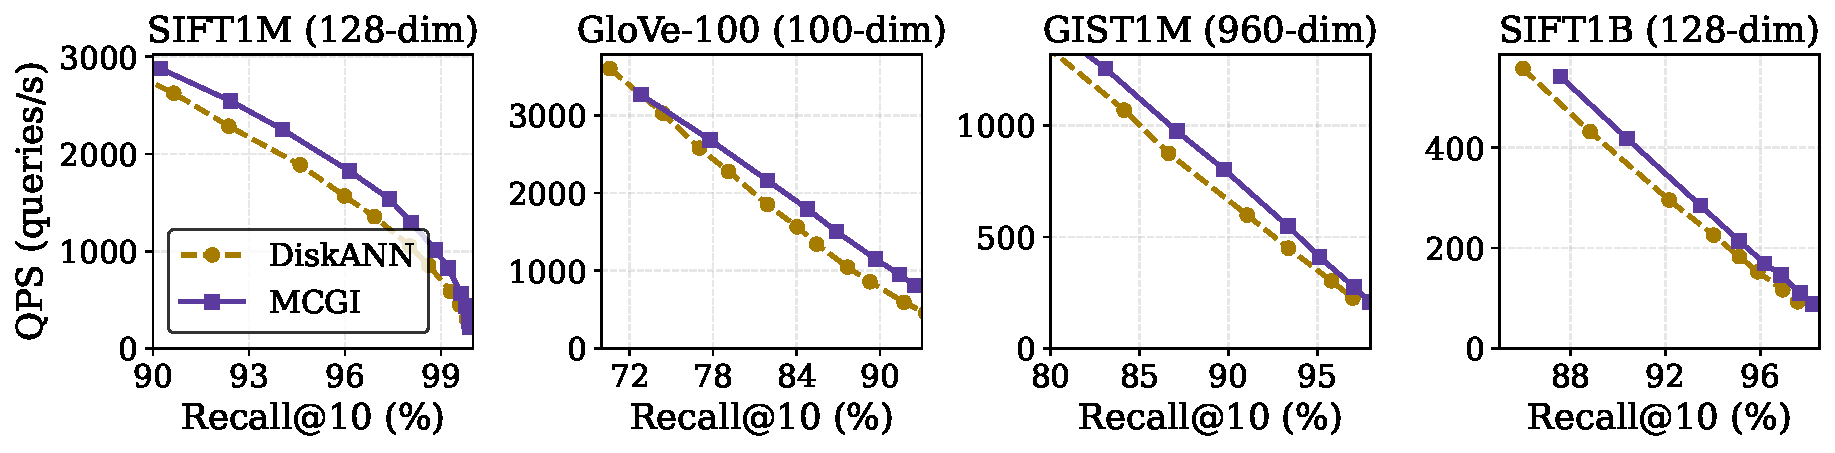
\includegraphics[width=\textwidth]{figures/recall_qps.pdf}
    \caption{Recall-QPS trade-off of \ours{} and DiskANN on the million-scale datasets.}
    \label{fig:results}
\end{figure*}

Figure~\ref{fig:results} plots the query throughput against Recall@10 for the two methods. \ours{} raises the throughput of DiskANN on all three million-scale datasets, and the improvement grows with the target recall. On SIFT1M, the gain rises from $1.15\times$ at 95\% recall to $1.33\times$ at 99\%. GloVe-100 and GIST1M follow the same trend, with gains from $1.12\times$ at 80\% to $1.43\times$ at 90\% and from $1.12\times$ at 85\% to $1.20\times$ at 95\%, respectively. The growth with recall agrees with Proposition~\ref{prop:fixed_beam}, because a high target recall forces a fixed search to use a long list for every query, including the many queries in low-LID regions that converge early. \ours{} shortens the lists of these queries and lengthens the lists of queries in high-LID regions, which removes disk reads that do not improve the result.

\subsection{Billion-scale Scalability}

We build one DiskANN index for each of SIFT1B and Deep1B with the standard sharded construction under a memory budget of 300 GiB. The construction splits the 8-bit vectors of SIFT1B into three overlapping shards and completes in 4.8 hours on the CPU cores of the platform, while the 32-bit vectors of Deep1B need seven shards and 5.4 hours. Both indexes use $R = 32$, $L_{build} = 50$, and 31-byte PQ codes, and both methods again search the same index. The calibration queries of each dataset are the even-indexed half of its 10{,}000 official queries, and the evaluation uses the odd-indexed half. The requested list sizes extend to $\bar{L} = 1{,}000$ on SIFT1B and to $\bar{L} = 2{,}000$ on Deep1B, since DiskANN needs a list longer than 400 on SIFT1B and longer than 800 on Deep1B to reach 95\% recall.

\begin{figure*}[t]
    \centering
    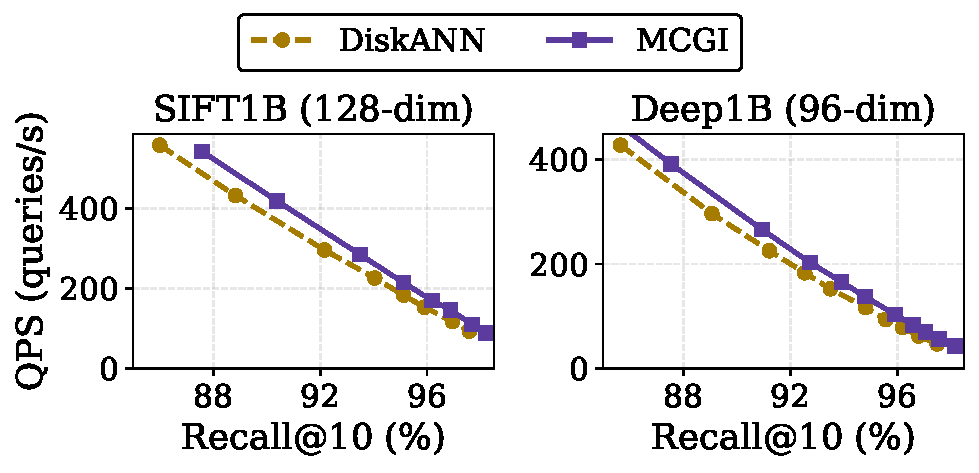
\includegraphics[width=0.49\textwidth]{figures/recall_qps_1b.pdf}
    \hfill
    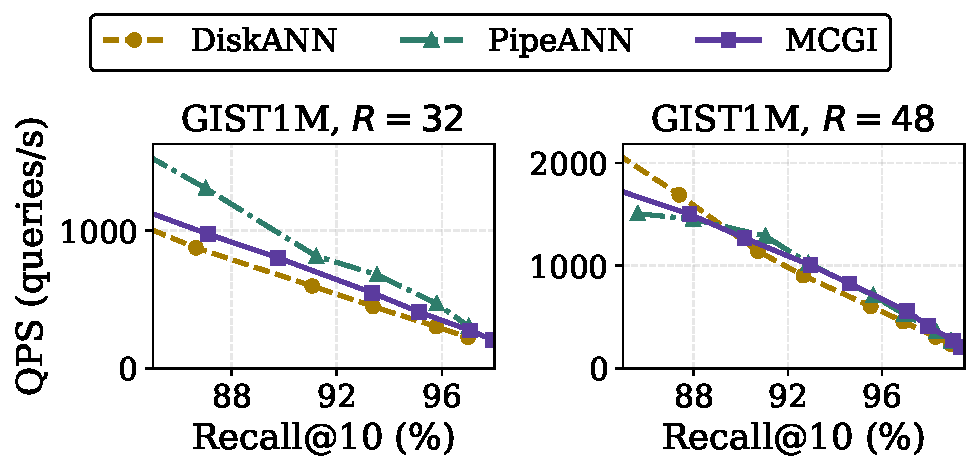
\includegraphics[width=0.49\textwidth]{figures/gist_compare.pdf}
    \caption{Recall-QPS at one billion vectors (left) and of disk-resident indexes on GIST1M (right).}
    \label{fig:results_1b}
    \label{fig:gist_compare}
\end{figure*}

The left two panels of Figure~\ref{fig:results_1b} show that the gain of \ours{} persists at one billion vectors on both datasets and again grows with the target recall. On SIFT1B, \ours{} raises the throughput of DiskANN from $1.07\times$ at 85\% recall to $1.17\times$ at 95\% and to $1.22\times$ at 97\%, where the throughput rises from 115 to 141 queries per second. Deep1B follows the same trend with gains from $1.08\times$ at 85\% to $1.18\times$ at 95\% and to $1.24\times$ at 97\%, where the throughput rises from 58 to 72 queries per second. At the longest list that we evaluate, DiskANN stays below 98\% recall on both datasets, whereas \ours{} reaches 98.2\% on each of them, at 89 queries per second on SIFT1B and 42 on Deep1B.

\subsection{Comparison with Pipelined and In-memory Search}

We compare \ours{} with PipeANN~\cite{osdi25pipeann, fast26odinann}, which overlaps the disk reads of each query in a pipelined beam search, on GIST1M with $R = 32$ and $R = 48$. PipeANN searches the same DiskANN index files as DiskANN and \ours{}, with 32 threads, its in-memory entry-point index built from a 1\% sample, and the better of the I/O widths 4 and 32. HNSW~\cite{malkov2018efficient}, IVF-Flat~\cite{johnson2019billion}, and CSPG~\cite{NEURIPS2024_bab1486c} serve as in-memory references, since they keep every full-precision vector in RAM.


\begin{wraptable}{r}{0.5\textwidth}
\vspace{-4mm}
\centering
\small
\setlength{\tabcolsep}{4pt}
\caption{GIST1M at 95\% Recall@10. $^\dagger$In memory.}
\label{tab:gist_compare}
\begin{tabular}{lcccc}
\toprule
 & \multicolumn{2}{c}{$R = 32$} & \multicolumn{2}{c}{$R = 48$} \\
\cmidrule(lr){2-3} \cmidrule(lr){4-5}
Method & QPS & Reads & QPS & Reads \\
\midrule
DiskANN & 351 & 272.7 & 659 & 146.7 \\
PipeANN & 545 & 268.3 & 780 & 143.8 \\
\ours{} & 420 & \textbf{223.7} & \textbf{785} & \textbf{125.5} \\
\midrule
CSPG$^\dagger$ & 5{,}742 & -- & 9{,}107 & -- \\
HNSW$^\dagger$ & 6{,}678 & -- & -- & -- \\
IVF-Flat$^\dagger$ & \multicolumn{4}{c}{1{,}292 (no degree bound)} \\
\bottomrule
\end{tabular}
\vspace{-3mm}
\end{wraptable}
The right two panels of Figure~\ref{fig:gist_compare} and Table~\ref{tab:gist_compare} show that \ours{} issues the fewest disk reads of the three disk-resident methods. At 95\% recall, \ours{} reads 224 nodes per query with $R = 32$ and 126 with $R = 48$, which is 13--18\% fewer than DiskANN and PipeANN, whose reads differ from each other by at most 2\%. PipeANN turns the same reads into higher throughput by overlapping them, and it leads at $R = 32$ with 545 queries per second against 420 for \ours{}. With $R = 48$, \ours{} matches PipeANN at 95\% recall with 785 against 780 queries per second and surpasses it at 97\% recall with 564 against 521. The two techniques act on different costs: PipeANN shortens the wait for each read, while \ours{} removes reads, so the query-adaptive list can also size the candidate list of a pipelined search. The in-memory indexes reach 1{,}292 to 9{,}107 queries per second at 95\% recall, at the price of holding the 3.84~GB of full-precision vectors in RAM, whereas the disk-resident methods hold mainly the 322~MB of PQ codes.

\subsection{Ablation and Sensitivity}

Figure~\ref{fig:ablation} attributes the gain of \ours{} at the highest target recall of each million-scale dataset, namely 99\% on SIFT1M, 90\% on GloVe-100, and 95\% on GIST1M. Each variant is fitted on the same calibration queries and searched once on the same index as DiskANN. The random variant keeps the fitted list sizes of \ours{} in distribution but assigns them to queries at random, which lowers the throughput to $0.72\times$--$0.84\times$ that of DiskANN. The gain therefore comes from matching each list to the geometry of its query, not from varying the list size. The two LID features alone retain gains of $1.18\times$--$1.33\times$, and the distance features alone, namely the first and tenth expanded distances and the candidate count, retain $1.25\times$--$1.37\times$, since the LID estimate is a function of the same distances.

\begin{figure*}[t]
    \centering
    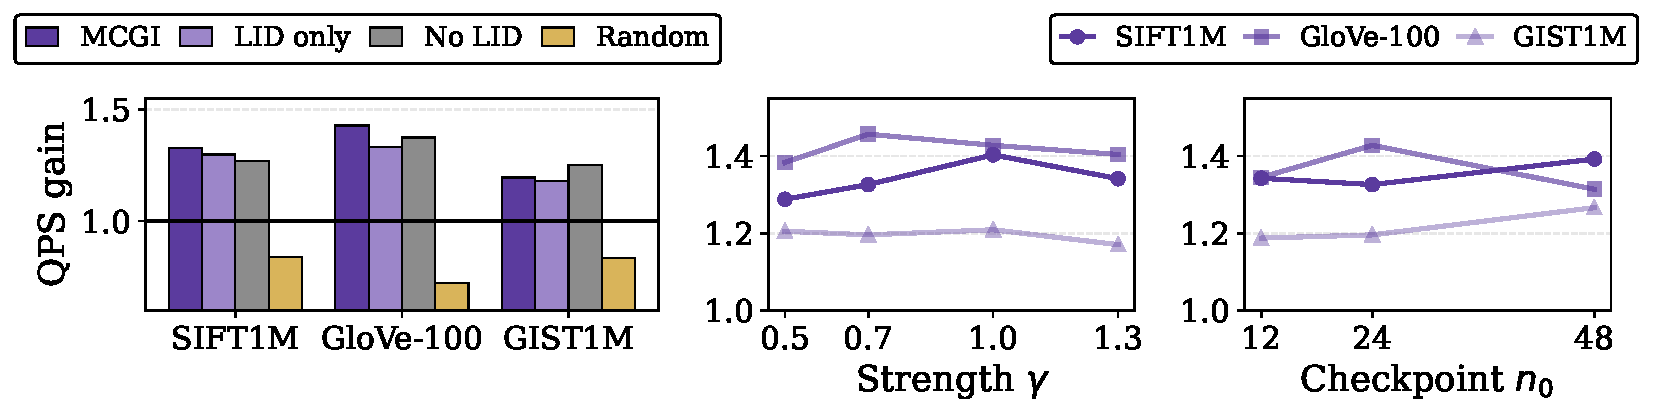
\includegraphics[width=\textwidth]{figures/ablation.pdf}
    \caption{QPS gain of \ours{} variants over DiskANN at the highest target recall of each dataset.}
    \label{fig:ablation}
\end{figure*}

The last two panels of Figure~\ref{fig:ablation} vary the strength $\gamma$ of Eq.~\eqref{eq:adaptive_list} from 0.5 to 1.3 and the checkpoint $n_0$ from 12 to 48 expansions around the calibrated setting. Every setting keeps a gain of at least $1.17\times$, and the calibrated setting stays within $0.08\times$ of the best setting on each dataset. The calibration therefore needs no careful tuning of either parameter, and the default $n_0 = 24$ serves all datasets.

\section{Conclusion}

This paper presents MCGI, a geometry-aware disk-resident indexing method for high-dimensional data of varying intrinsic dimensionality.
MCGI addresses the Euclidean-Geodesic mismatch by adapting the candidate list of each query, and optionally the pruning parameter of each node, to local intrinsic dimensionality, where the list size follows from distances that the search has already computed. Our theoretical analysis shows that the success probability of any fixed beam width decays exponentially with the LID of the query, and the query-adaptive list approximates the iso-recall schedule from distances that the search has already computed. At matched high recall, MCGI raises the throughput of DiskANN by up to $1.43\times$ on benchmarks of 96 to 960 dimensions and by up to $1.24\times$ at one billion vectors.

% Our future work will explore several promising directions. First, we plan to extend the MCGI framework to support dynamic updates, enabling efficient insertions and deletions while maintaining manifold-consistent routing. Second, we aim to investigate more sophisticated geometric metrics beyond LID, such as curvature or local density estimates, to further refine the pruning strategy. Finally, we will explore the integration of MCGI with emerging hardware accelerators (e.g., NVMe SSDs with built-in compute capabilities) to push the boundaries of disk-resident indexing performance.

\begin{ack}
Results presented in this paper were obtained using the Chameleon testbed supported by the National Science Foundation.
The author appreciates the feedback and praise from early users around the world (e.g., South Korea, New Zealand) of MCGI and AdaDisk (the parent project of MCGI), without which the author would not have been able to continue improving the system and pushing the performance boundary.
Copilot and Claude assisted with the system implementation, the experiments, and the writing of this paper; the author verified all results and takes full responsibility for the content. 

The source code of MCGI is available at \url{https://github.com/hpdic/mcgi}. 
\end{ack}

\bibliography{ref}
\bibliographystyle{plain}

\clearpage
\section*{NeurIPS Paper Checklist}

%%% BEGIN INSTRUCTIONS %%%
% The checklist is designed to encourage best practices for responsible machine learning research, addressing issues of reproducibility, transparency, research ethics, and societal impact. Do not remove the checklist: {\bf The papers not including the checklist will be desk rejected.} The checklist should follow the references and follow the (optional) supplemental material.  The checklist does NOT count towards the page
% limit. 

% Please read the checklist guidelines carefully for information on how to answer these questions. For each question in the checklist:
% \begin{itemize}
%     \item You should answer \answerYes{}, \answerNo{}, or \answerNA{}.
%     \item \answerNA{} means either that the question is Not Applicable for that particular paper or the relevant information is Not Available.
%     \item Please provide a short (1--2 sentence) justification right after your answer (even for \answerNA). 
%    % \item {\bf The papers not including the checklist will be desk rejected.}
% \end{itemize}

% {\bf The checklist answers are an integral part of your paper submission.} They are visible to the reviewers, area chairs, senior area chairs, and ethics reviewers. You will also be asked to include it (after eventual revisions) with the final version of your paper, and its final version will be published with the paper.

% The reviewers of your paper will be asked to use the checklist as one of the factors in their evaluation. While \answerYes{} is generally preferable to \answerNo{}, it is perfectly acceptable to answer \answerNo{} provided a proper justification is given (e.g., error bars are not reported because it would be too computationally expensive'' or ``we were unable to find the license for the dataset we used''). In general, answering \answerNo{} or \answerNA{} is not grounds for rejection. While the questions are phrased in a binary way, we acknowledge that the true answer is often more nuanced, so please just use your best judgment and write a justification to elaborate. All supporting evidence can appear either in the main paper or the supplemental material, provided in appendix. If you answer \answerYes{} to a question, in the justification please point to the section(s) where related material for the question can be found.

% IMPORTANT, please:
% \begin{itemize}
%     \item {\bf Delete this instruction block, but keep the section heading ``NeurIPS Paper Checklist"},
%     \item  {\bf Keep the checklist subsection headings, questions/answers and guidelines below.}
%     \item {\bf Do not modify the questions and only use the provided macros for your answers}.
% \end{itemize} 
 

%%% END INSTRUCTIONS %%%


\begin{enumerate}

\item {\bf Claims}
    \item[] Question: Do the main claims made in the abstract and introduction accurately reflect the paper's contributions and scope?
    \item[] Answer: \answerYes{} % Replace by \answerYes{}, \answerNo{}, or \answerNA{}.
    \item[] Justification: The paper presents both theoretical and experimental evidence to support its claims.
    \item[] Guidelines:
    \begin{itemize}
        \item The answer \answerNA{} means that the abstract and introduction do not include the claims made in the paper.
        \item The abstract and/or introduction should clearly state the claims made, including the contributions made in the paper and important assumptions and limitations. A \answerNo{} or \answerNA{} answer to this question will not be perceived well by the reviewers. 
        \item The claims made should match theoretical and experimental results, and reflect how much the results can be expected to generalize to other settings. 
        \item It is fine to include aspirational goals as motivation as long as it is clear that these goals are not attained by the paper. 
    \end{itemize}

\item {\bf Limitations}
    \item[] Question: Does the paper discuss the limitations of the work performed by the authors?
    \item[] Answer: \answerYes{} % Replace by \answerYes{}, \answerNo{}, or \answerNA{}.
    \item[] Justification: Appendix~\ref{appendix:limitations} discusses the scope of the evaluated mechanism, the effect of the degree bound on the construction-time rule, the tail latency of the adaptive list, the calibration requirements, and the modeling assumptions of the theory.
    \item[] Guidelines:
    \begin{itemize}
        \item The answer \answerNA{} means that the paper has no limitation while the answer \answerNo{} means that the paper has limitations, but those are not discussed in the paper. 
        \item The authors are encouraged to create a separate ``Limitations'' section in their paper.
        \item The paper should point out any strong assumptions and how robust the results are to violations of these assumptions (e.g., independence assumptions, noiseless settings, model well-specification, asymptotic approximations only holding locally). The authors should reflect on how these assumptions might be violated in practice and what the implications would be.
        \item The authors should reflect on the scope of the claims made, e.g., if the approach was only tested on a few datasets or with a few runs. In general, empirical results often depend on implicit assumptions, which should be articulated.
        \item The authors should reflect on the factors that influence the performance of the approach. For example, a facial recognition algorithm may perform poorly when image resolution is low or images are taken in low lighting. Or a speech-to-text system might not be used reliably to provide closed captions for online lectures because it fails to handle technical jargon.
        \item The authors should discuss the computational efficiency of the proposed algorithms and how they scale with dataset size.
        \item If applicable, the authors should discuss possible limitations of their approach to address problems of privacy and fairness.
        \item While the authors might fear that complete honesty about limitations might be used by reviewers as grounds for rejection, a worse outcome might be that reviewers discover limitations that aren't acknowledged in the paper. The authors should use their best judgment and recognize that individual actions in favor of transparency play an important role in developing norms that preserve the integrity of the community. Reviewers will be specifically instructed to not penalize honesty concerning limitations.
    \end{itemize}

\item {\bf Theory assumptions and proofs}
    \item[] Question: For each theoretical result, does the paper provide the full set of assumptions and a complete (and correct) proof?
    \item[] Answer: \answerYes{} % Replace by \answerYes{}, \answerNo{}, or \answerNA{}.
    \item[] Justification: Every proposition states its assumptions, including the absence of a degree bound where it matters, and Appendix~\ref{appendix:proofs} gives the full proofs; Appendix~\ref{appendix:limitations} lists the modeling assumptions of the analysis.
    \item[] Guidelines:
    \begin{itemize}
        \item The answer \answerNA{} means that the paper does not include theoretical results. 
        \item All the theorems, formulas, and proofs in the paper should be numbered and cross-referenced.
        \item All assumptions should be clearly stated or referenced in the statement of any theorems.
        \item The proofs can either appear in the main paper or the supplemental material, but if they appear in the supplemental material, the authors are encouraged to provide a short proof sketch to provide intuition. 
        \item Inversely, any informal proof provided in the core of the paper should be complemented by formal proofs provided in appendix or supplemental material.
        \item Theorems and Lemmas that the proof relies upon should be properly referenced. 
    \end{itemize}

 \item {\bf Experimental result reproducibility}
    \item[] Question: Does the paper fully disclose all the information needed to reproduce the main experimental results of the paper to the extent that it affects the main claims and/or conclusions of the paper (regardless of whether the code and data are provided or not)?
    \item[] Answer: \answerYes{} % Replace by \answerYes{}, \answerNo{}, or \answerNA{}.
    \item[] Justification: The code, the experiment scripts, and the data behind every figure are available in the public repository \url{https://github.com/hpdic/mcgi}, and Section~\ref{sec:experiments} and Appendix~\ref{appendix:setup} describe the setup.
    \item[] Guidelines:
    \begin{itemize}
        \item The answer \answerNA{} means that the paper does not include experiments.
        \item If the paper includes experiments, a \answerNo{} answer to this question will not be perceived well by the reviewers: Making the paper reproducible is important, regardless of whether the code and data are provided or not.
        \item If the contribution is a dataset and\slash or model, the authors should describe the steps taken to make their results reproducible or verifiable. 
        \item Depending on the contribution, reproducibility can be accomplished in various ways. For example, if the contribution is a novel architecture, describing the architecture fully might suffice, or if the contribution is a specific model and empirical evaluation, it may be necessary to either make it possible for others to replicate the model with the same dataset, or provide access to the model. In general. releasing code and data is often one good way to accomplish this, but reproducibility can also be provided via detailed instructions for how to replicate the results, access to a hosted model (e.g., in the case of a large language model), releasing of a model checkpoint, or other means that are appropriate to the research performed.
        \item While NeurIPS does not require releasing code, the conference does require all submissions to provide some reasonable avenue for reproducibility, which may depend on the nature of the contribution. For example
        \begin{enumerate}
            \item If the contribution is primarily a new algorithm, the paper should make it clear how to reproduce that algorithm.
            \item If the contribution is primarily a new model architecture, the paper should describe the architecture clearly and fully.
            \item If the contribution is a new model (e.g., a large language model), then there should either be a way to access this model for reproducing the results or a way to reproduce the model (e.g., with an open-source dataset or instructions for how to construct the dataset).
            \item We recognize that reproducibility may be tricky in some cases, in which case authors are welcome to describe the particular way they provide for reproducibility. In the case of closed-source models, it may be that access to the model is limited in some way (e.g., to registered users), but it should be possible for other researchers to have some path to reproducing or verifying the results.
        \end{enumerate}
    \end{itemize}


\item {\bf Open access to data and code}
    \item[] Question: Does the paper provide open access to the data and code, with sufficient instructions to faithfully reproduce the main experimental results, as described in supplemental material?
    \item[] Answer: \answerYes{} % Replace by \answerYes{}, \answerNo{}, or \answerNA{}.
    \item[] Justification: The public repository \url{https://github.com/hpdic/mcgi} contains the code, the experiment scripts, and the exported results; all datasets are public benchmarks.
    \item[] Guidelines:
    \begin{itemize}
        \item The answer \answerNA{} means that paper does not include experiments requiring code.
        \item Please see the NeurIPS code and data submission guidelines (\url{https://neurips.cc/public/guides/CodeSubmissionPolicy}) for more details.
        \item While we encourage the release of code and data, we understand that this might not be possible, so \answerNo{} is an acceptable answer. Papers cannot be rejected simply for not including code, unless this is central to the contribution (e.g., for a new open-source benchmark).
        \item The instructions should contain the exact command and environment needed to run to reproduce the results. See the NeurIPS code and data submission guidelines (\url{https://neurips.cc/public/guides/CodeSubmissionPolicy}) for more details.
        \item The authors should provide instructions on data access and preparation, including how to access the raw data, preprocessed data, intermediate data, and generated data, etc.
        \item The authors should provide scripts to reproduce all experimental results for the new proposed method and baselines. If only a subset of experiments are reproducible, they should state which ones are omitted from the script and why.
        \item At submission time, to preserve anonymity, the authors should release anonymized versions (if applicable).
        \item Providing as much information as possible in supplemental material (appended to the paper) is recommended, but including URLs to data and code is permitted.
    \end{itemize}


\item {\bf Experimental setting/details}
    \item[] Question: Does the paper specify all the training and test details (e.g., data splits, hyperparameters, how they were chosen, type of optimizer) necessary to understand the results?
    \item[] Answer: \answerYes{} % Replace by \answerYes{}, \answerNo{}, or \answerNA{}.
    \item[] Justification: Section~\ref{sec:experiments} and Appendix~\ref{appendix:setup} give the datasets, the index and search parameters, the calibration protocol, and the baseline configurations.
    \item[] Guidelines:
    \begin{itemize}
        \item The answer \answerNA{} means that the paper does not include experiments.
        \item The experimental setting should be presented in the core of the paper to a level of detail that is necessary to appreciate the results and make sense of them.
        \item The full details can be provided either with the code, in appendix, or as supplemental material.
    \end{itemize}

\item {\bf Experiment statistical significance}
    \item[] Question: Does the paper report error bars suitably and correctly defined or other appropriate information about the statistical significance of the experiments?
    \item[] Answer: \answerNo{} % Replace by \answerYes{}, \answerNo{}, or \answerNA{}.
    \item[] Justification: Each configuration runs once on an otherwise idle machine with the page cache dropped, and both methods search the same index with the same queries; the paper does not report error bars.
    \item[] Guidelines:
    \begin{itemize}
        \item The answer \answerNA{} means that the paper does not include experiments.
        \item The authors should answer \answerYes{} if the results are accompanied by error bars, confidence intervals, or statistical significance tests, at least for the experiments that support the main claims of the paper.
        \item The factors of variability that the error bars are capturing should be clearly stated (for example, train/test split, initialization, random drawing of some parameter, or overall run with given experimental conditions).
        \item The method for calculating the error bars should be explained (closed form formula, call to a library function, bootstrap, etc.)
        \item The assumptions made should be given (e.g., Normally distributed errors).
        \item It should be clear whether the error bar is the standard deviation or the standard error of the mean.
        \item It is OK to report 1-sigma error bars, but one should state it. The authors should preferably report a 2-sigma error bar than state that they have a 96\% CI, if the hypothesis of Normality of errors is not verified.
        \item For asymmetric distributions, the authors should be careful not to show in tables or figures symmetric error bars that would yield results that are out of range (e.g., negative error rates).
        \item If error bars are reported in tables or plots, the authors should explain in the text how they were calculated and reference the corresponding figures or tables in the text.
    \end{itemize}

\item {\bf Experiments compute resources}
    \item[] Question: For each experiment, does the paper provide sufficient information on the computer resources (type of compute workers, memory, time of execution) needed to reproduce the experiments?
    \item[] Answer: \answerYes{} % Replace by \answerYes{}, \answerNo{}, or \answerNA{}.
    \item[] Justification: Section~\ref{sec:experiments} and Appendix~\ref{appendix:setup} describe the platform (192 virtual cores, 960 GiB of RAM, and a virtual block device), and Table~\ref{tab:offline_cost} reports the build and calibration times.
    \item[] Guidelines:
    \begin{itemize}
        \item The answer \answerNA{} means that the paper does not include experiments.
        \item The paper should indicate the type of compute workers CPU or GPU, internal cluster, or cloud provider, including relevant memory and storage.
        \item The paper should provide the amount of compute required for each of the individual experimental runs as well as estimate the total compute. 
        \item The paper should disclose whether the full research project required more compute than the experiments reported in the paper (e.g., preliminary or failed experiments that didn't make it into the paper). 
    \end{itemize}
    
\item {\bf Code of ethics}
    \item[] Question: Does the research conducted in the paper conform, in every respect, with the NeurIPS Code of Ethics \url{https://neurips.cc/public/EthicsGuidelines}?
    \item[] Answer: \answerYes{} % Replace by \answerYes{}, \answerNo{}, or \answerNA{}.
    \item[] Justification: We believe we have followed the NeurIPS Code of Ethics in all aspects of our research.
    \item[] Guidelines:
    \begin{itemize}
        \item The answer \answerNA{} means that the authors have not reviewed the NeurIPS Code of Ethics.
        \item If the authors answer \answerNo, they should explain the special circumstances that require a deviation from the Code of Ethics.
        \item The authors should make sure to preserve anonymity (e.g., if there is a special consideration due to laws or regulations in their jurisdiction).
    \end{itemize}


\item {\bf Broader impacts}
    \item[] Question: Does the paper discuss both potential positive societal impacts and negative societal impacts of the work performed?
    \item[] Answer: \answerNA{} % Replace by \answerYes{}, \answerNo{}, or \answerNA{}.
    \item[] Justification: The paper studies the efficiency of nearest-neighbor search over public benchmarks and has no direct societal impact beyond faster retrieval.
    \item[] Guidelines:
    \begin{itemize}
        \item The answer \answerNA{} means that there is no societal impact of the work performed.
        \item If the authors answer \answerNA{} or \answerNo, they should explain why their work has no societal impact or why the paper does not address societal impact.
        \item Examples of negative societal impacts include potential malicious or unintended uses (e.g., disinformation, generating fake profiles, surveillance), fairness considerations (e.g., deployment of technologies that could make decisions that unfairly impact specific groups), privacy considerations, and security considerations.
        \item The conference expects that many papers will be foundational research and not tied to particular applications, let alone deployments. However, if there is a direct path to any negative applications, the authors should point it out. For example, it is legitimate to point out that an improvement in the quality of generative models could be used to generate Deepfakes for disinformation. On the other hand, it is not needed to point out that a generic algorithm for optimizing neural networks could enable people to train models that generate Deepfakes faster.
        \item The authors should consider possible harms that could arise when the technology is being used as intended and functioning correctly, harms that could arise when the technology is being used as intended but gives incorrect results, and harms following from (intentional or unintentional) misuse of the technology.
        \item If there are negative societal impacts, the authors could also discuss possible mitigation strategies (e.g., gated release of models, providing defenses in addition to attacks, mechanisms for monitoring misuse, mechanisms to monitor how a system learns from feedback over time, improving the efficiency and accessibility of ML).
    \end{itemize}
    
\item {\bf Safeguards}
    \item[] Question: Does the paper describe safeguards that have been put in place for responsible release of data or models that have a high risk for misuse (e.g., pre-trained language models, image generators, or scraped datasets)?
    \item[] Answer: \answerNA{} % Replace by \answerYes{}, \answerNo{}, or \answerNA{}.
    \item[] Justification: The paper releases no data or model with a risk of misuse.
    \item[] Guidelines:
    \begin{itemize}
        \item The answer \answerNA{} means that the paper poses no such risks.
        \item Released models that have a high risk for misuse or dual-use should be released with necessary safeguards to allow for controlled use of the model, for example by requiring that users adhere to usage guidelines or restrictions to access the model or implementing safety filters. 
        \item Datasets that have been scraped from the Internet could pose safety risks. The authors should describe how they avoided releasing unsafe images.
        \item We recognize that providing effective safeguards is challenging, and many papers do not require this, but we encourage authors to take this into account and make a best faith effort.
    \end{itemize}

\item {\bf Licenses for existing assets}
    \item[] Question: Are the creators or original owners of assets (e.g., code, data, models), used in the paper, properly credited and are the license and terms of use explicitly mentioned and properly respected?
    \item[] Answer: \answerYes{} % Replace by \answerYes{}, \answerNo{}, or \answerNA{}.
    \item[] Justification: The paper cites the creators of every dataset (SIFT1M, GIST1M, SIFT1B, GloVe-100, and Deep1B) and every baseline. DiskANN and Faiss are released under the MIT license, PipeANN and hnswlib under the Apache License 2.0, and CSPG is used from the public repository of its authors for research comparison; the datasets are public benchmarks used under the terms of their original releases.
    \item[] Guidelines:
    \begin{itemize}
        \item The answer \answerNA{} means that the paper does not use existing assets.
        \item The authors should cite the original paper that produced the code package or dataset.
        \item The authors should state which version of the asset is used and, if possible, include a URL.
        \item The name of the license (e.g., CC-BY 4.0) should be included for each asset.
        \item For scraped data from a particular source (e.g., website), the copyright and terms of service of that source should be provided.
        \item If assets are released, the license, copyright information, and terms of use in the package should be provided. For popular datasets, \url{paperswithcode.com/datasets} has curated licenses for some datasets. Their licensing guide can help determine the license of a dataset.
        \item For existing datasets that are re-packaged, both the original license and the license of the derived asset (if it has changed) should be provided.
        \item If this information is not available online, the authors are encouraged to reach out to the asset's creators.
    \end{itemize}

\item {\bf New assets}
    \item[] Question: Are new assets introduced in the paper well documented and is the documentation provided alongside the assets?
    \item[] Answer: \answerYes{} % Replace by \answerYes{}, \answerNo{}, or \answerNA{}.
    \item[] Justification: The code of \ours{} is released at \url{https://github.com/hpdic/mcgi} under the MIT license of its DiskANN code base, with a README that maps every figure and table to its script.
    \item[] Guidelines:
    \begin{itemize}
        \item The answer \answerNA{} means that the paper does not release new assets.
        \item Researchers should communicate the details of the dataset\slash code\slash model as part of their submissions via structured templates. This includes details about training, license, limitations, etc. 
        \item The paper should discuss whether and how consent was obtained from people whose asset is used.
        \item At submission time, remember to anonymize your assets (if applicable). You can either create an anonymized URL or include an anonymized zip file.
    \end{itemize}

\item {\bf Crowdsourcing and research with human subjects}
    \item[] Question: For crowdsourcing experiments and research with human subjects, does the paper include the full text of instructions given to participants and screenshots, if applicable, as well as details about compensation (if any)? 
    \item[] Answer: \answerNA{} % Replace by \answerYes{}, \answerNo{}, or \answerNA{}.
    \item[] Justification: The paper involves no crowdsourcing or human subjects.
    \item[] Guidelines:
    \begin{itemize}
        \item The answer \answerNA{} means that the paper does not involve crowdsourcing nor research with human subjects.
        \item Including this information in the supplemental material is fine, but if the main contribution of the paper involves human subjects, then as much detail as possible should be included in the main paper. 
        \item According to the NeurIPS Code of Ethics, workers involved in data collection, curation, or other labor should be paid at least the minimum wage in the country of the data collector. 
    \end{itemize}

\item {\bf Institutional review board (IRB) approvals or equivalent for research with human subjects}
    \item[] Question: Does the paper describe potential risks incurred by study participants, whether such risks were disclosed to the subjects, and whether Institutional Review Board (IRB) approvals (or an equivalent approval/review based on the requirements of your country or institution) were obtained?
    \item[] Answer: \answerNA{} % Replace by \answerYes{}, \answerNo{}, or \answerNA{}.
    \item[] Justification: The paper involves no human subjects.
    \item[] Guidelines:
    \begin{itemize}
        \item The answer \answerNA{} means that the paper does not involve crowdsourcing nor research with human subjects.
        \item Depending on the country in which research is conducted, IRB approval (or equivalent) may be required for any human subjects research. If you obtained IRB approval, you should clearly state this in the paper. 
        \item We recognize that the procedures for this may vary significantly between institutions and locations, and we expect authors to adhere to the NeurIPS Code of Ethics and the guidelines for their institution. 
        \item For initial submissions, do not include any information that would break anonymity (if applicable), such as the institution conducting the review.
    \end{itemize}

\item {\bf Declaration of LLM usage}
    \item[] Question: Does the paper describe the usage of LLMs if it is an important, original, or non-standard component of the core methods in this research? Note that if the LLM is used only for writing, editing, or formatting purposes and does \emph{not} impact the core methodology, scientific rigor, or originality of the research, declaration is not required.
    %this research? 
    \item[] Answer: \answerNA{} % Replace by \answerYes{}, \answerNo{}, or \answerNA{}.
    \item[] Justification: LLMs assisted with the implementation, the experiments, and the writing, as stated in the acknowledgments, but they are not a component of the method.
    \item[] Guidelines:
    \begin{itemize}
        \item The answer \answerNA{} means that the core method development in this research does not involve LLMs as any important, original, or non-standard components.
        \item Please refer to our LLM policy in the NeurIPS handbook for what should or should not be described.
    \end{itemize}

\end{enumerate}

\clearpage
\appendix

\section{Technical appendices and supplementary material}

\subsection{Complete Proofs}
\label{appendix:proofs}

\begin{proposition}[Monotonicity]\label{proof:mono}
The mapping function $\Phi$ is strictly increasing with respect to the estimated local intrinsic dimensionality. Formally, given that the standard deviation of the LID estimates $\sigma_{\widehat{\text{LID}}} > 0$ and the pruning range $\alpha_{\max} > \alpha_{\min}$, the derivative satisfies:
\begin{equation}
    \frac{d \Phi}{d \widehat{\text{LID}}(u)} > 0.
\end{equation}
\end{proposition}

\begin{proof}
Let $L = \widehat{\text{LID}}(u)$ be the independent variable. We define the normalized Z-score $z$ as a function of $L$:
\begin{equation}
    z(L) = \frac{L - \mu_{\widehat{\text{LID}}}}{\sigma_{\widehat{\text{LID}}}}.
\end{equation}
The mapping function is defined as:
\begin{equation}
    \Phi(L) = \alpha_{\min} + \frac{C}{1 + \exp(-z(L))},
\end{equation}
where $C = \alpha_{\max} - \alpha_{\min}$. Since we strictly require $\alpha_{\max} > \alpha_{\min}$, it follows that $C > 0$.
To determine the sign of the gradient, we apply the chain rule:
\begin{equation}
    \frac{d \Phi}{d L} = \frac{d \Phi}{d z} \cdot \frac{d z}{d L}.
\end{equation}
First, we differentiate the Z-score term with respect to $L$:
\begin{equation}
    \frac{d z}{d L} = \frac{1}{\sigma_{\widehat{\text{LID}}}}.
\end{equation}
Next, we differentiate the logistic component $\Phi$ with respect to $z$:
\begin{align}
    \frac{d \Phi}{d z} &= \frac{d}{d z} \left( \alpha_{\min} + C (1 + e^{-z})^{-1} \right) \\
    &= C \cdot (-1) \cdot (1 + e^{-z})^{-2} \cdot \frac{d}{d z}(1 + e^{-z}) \\
    &= C \cdot \frac{e^{-z}}{(1 + e^{-z})^2}.
\end{align}
Combining these terms yields the full derivative:
\begin{equation}
    \frac{d \Phi}{d L} = \frac{C}{\sigma_{\widehat{\text{LID}}}} \cdot \frac{e^{-z}}{(1 + e^{-z})^2}.
\end{equation}
We analyze the sign of each component:
\begin{itemize}
    \item The operational range constant $C > 0$.
    \item The standard deviation $\sigma_{\widehat{\text{LID}}} > 0$, assuming the dataset exhibits non-zero geometric variance.
    \item The exponential function $e^{-z} > 0$ for all $z \in \mathbb{R}$.
    \item The denominator $(1 + e^{-z})^2 > 0$.
\end{itemize}
Therefore, the derivative $\frac{d \Phi}{d L} = \frac{C}{\sigma_{\widehat{\text{LID}}}} \frac{e^{-z}}{(1 + e^{-z})^2}$ is strictly positive.
This confirms that the pruning parameter $\alpha$ strictly increases with the local geometric complexity, thereby enforcing a more conservative pruning that retains more navigational edges in high-LID regions.
\end{proof}

\begin{proposition}[Boundedness]\label{proof:bound}
The pruning parameter $\alpha(u)$ derived from the mapping function is strictly bounded within the prescribed operational interval. For any node $u$ with a finite LID estimate:
\begin{equation}
    \alpha_{\min} < \alpha(u) < \alpha_{\max}.
\end{equation}
\end{proposition}

\begin{proof}
Let $S(u)$ denote the logistic component of the mapping function:
\begin{equation}
    S(u) = \frac{1}{1 + \exp(-z(u))}.
\end{equation}
For any finite input $\widehat{\text{LID}}(u)$, the Z-score $z(u)$ is finite. The exponential function maps the real line to the positive real line, i.e., $\exp(-z(u)) \in (0, \infty)$.
Consequently, the denominator lies in the interval $(1, \infty)$. Taking the reciprocal yields the bounds for the logistic component:
\begin{equation}
    0 < S(u) < 1.
\end{equation}
Substituting $S(u)$ back into the definition of $\Phi$:
\begin{equation}
    \alpha(u) = \alpha_{\min} + (\alpha_{\max} - \alpha_{\min}) \cdot S(u).
\end{equation}
Since $(\alpha_{\max} - \alpha_{\min}) > 0$, we can apply the inequality boundaries:
\begin{align}
    \alpha(u) &> \alpha_{\min} + (\alpha_{\max} - \alpha_{\min}) \cdot 0 = \alpha_{\min}, \\
    \alpha(u) &< \alpha_{\min} + (\alpha_{\max} - \alpha_{\min}) \cdot 1 = \alpha_{\max}.
\end{align}
This proves that the topology is strictly confined. 
The pruning behavior never exceeds the relaxation upper limit ($\alpha_{\max}$) and never becomes stricter than the lower limit ($\alpha_{\min}$), ensuring graph connectivity and preventing degree explosion.
\end{proof}

\begin{lemma}[Local Complexity Lower Bound]
\label{proof:complexity}
Consistent with the complexity bounds established for growth-restricted metrics~\cite{karger2002finding}, for a query $q$ on a manifold $\mathcal{M}$, the expected number of distance evaluations $N_{dist}$ required for successful greedy routing scales exponentially with the local intrinsic dimensionality $d = \text{LID}(q)$:
\begin{equation}
    \mathbb{E}[N_{dist}] \ge \Omega\left( \sqrt{d} \cdot \exp(\lambda \cdot d) \right),
\end{equation}
where $\lambda > 0$ is a geometric constant derived from the required convergence rate.
\end{lemma}

\begin{proof}
Let the local dataset around a query $q$ be modeled as a uniform distribution on a manifold of intrinsic dimension $d$. Consider a greedy routing step where the algorithm is currently at a node $u$ with distance $r = \|u - q\|$.

\paragraph{1. Geometric Condition for Improvement.}
To make progress, the algorithm must identify a neighbor $v$ such that the distance to the query is reduced by a factor $\epsilon$ (where $0 < \epsilon < 1$), i.e., $\|v - q\| \le (1-\epsilon)r$.
Let $s = \|u - v\|$ be the distance between the current node and the candidate neighbor (the step size). Applying the Law of Cosines to triangle $\triangle u v q$, we have:
\begin{equation}
    \|v - q\|^2 = r^2 + s^2 - 2rs \cos \theta,
\end{equation}
where $\theta$ is the angle between the vector $\vec{u q}$ and $\vec{u v}$. The improvement condition $\|v - q\|^2 \le (1-\epsilon)^2 r^2$ implies:
\begin{align}
    r^2 + s^2 - 2rs \cos \theta &\le (1-\epsilon)^2 r^2, \nonumber \\
    2rs \cos \theta &\ge r^2 + s^2 - r^2(1-\epsilon)^2, \nonumber \\
    \cos \theta &\ge \frac{r^2 + s^2 - r^2(1-\epsilon)^2}{2rs}.
\end{align}
Assuming the step size is small relative to the distance (i.e., $s \ll r$), the right-hand side is dominated by $1 - (1-\epsilon)^2 \approx 2\epsilon$, yielding a critical angle threshold $\theta_{max}$ such that any successful neighbor must fall within the cone defined by $0 \le \theta \le \theta_{max}$.

\paragraph{2. Volume Concentration of the Improving Region.}
In the tangent space at $u$, the directions of neighbors are uniformly distributed on the unit hypersphere $\mathbb{S}^{d-1}$. The probability $P_{success}$ of finding a neighbor in the improving cone corresponds to the ratio of the surface area of the spherical cap $\mathcal{C}(\theta_{max})$ to the total surface area of $\mathbb{S}^{d-1}$.
This ratio is given by the regularized incomplete beta function, which can be expressed in terms of the integral over the polar angle $\phi$:
\begin{equation}
    P_{success} = \frac{\text{Area}(\mathcal{C}(\theta_{max}))}{\text{Area}(\mathbb{S}^{d-1})} = \frac{\int_0^{\theta_{max}} \sin^{d-2} \phi \, d\phi}{\int_0^{\pi} \sin^{d-2} \phi \, d\phi}.
\end{equation}

\paragraph{3. Asymptotic Analysis.}
We analyze the asymptotic behavior of this ratio as $d \to \infty$. The denominator relates to the surface area of the hypersphere and can be evaluated using the standard integral identity for powers of sine. Exploiting the symmetry of $\sin \phi$ around $\pi/2$, we have:
\begin{align}
    \int_0^{\pi} \sin^{d-2} \phi \, d\phi &= 2 \int_0^{\frac{\pi}{2}} \sin^{d-2} \phi \, d\phi \nonumber \\
    &= 2 \cdot \frac{\sqrt{\pi}}{2} \frac{\Gamma(\frac{d-1}{2})}{\Gamma(\frac{d}{2})} = \sqrt{\pi} \frac{\Gamma(\frac{d-1}{2})}{\Gamma(\frac{d}{2})}.
\end{align}
For high-dimensional spaces ($d \gg 1$), we apply the asymptotic property of the Gamma function ratio, $\frac{\Gamma(x+a)}{\Gamma(x)} \approx x^a$. Setting $x = d/2$ and $a = -1/2$, we obtain the approximation:
\begin{equation}
    \sqrt{\pi} \frac{\Gamma(\frac{d}{2} - \frac{1}{2})}{\Gamma(\frac{d}{2})} \approx \sqrt{\pi} \left( \frac{d}{2} \right)^{-\frac{1}{2}} = \sqrt{\frac{2\pi}{d}}.
\end{equation}
For the numerator, we exploit the concentration of measure near the integration boundary $\theta_{max}$. Since the integrand $\sin^{d-2} \phi$ decays exponentially fast away from $\theta_{max}$, the integral is dominated by the contribution near the upper limit. We apply integration by parts to extract the leading order term. 
Recall that $\frac{d}{d\phi}(\sin^{d-1} \phi) = (d-1)\sin^{d-2} \phi \cos \phi$. We rewrite the integrand as:
\begin{equation}
    \int_0^{\theta_{max}} \sin^{d-2} \phi \, d\phi = \int_0^{\theta_{max}} \frac{1}{(d-1)\cos \phi} \frac{d}{d\phi}(\sin^{d-1} \phi) \, d\phi.
\end{equation}
Neglecting lower-order terms generated by the derivative of $\frac{1}{\cos \phi}$, the integral approximates to the boundary term:
\begin{equation}
    \left[ \frac{\sin^{d-1} \phi}{(d-1)\cos \phi} \right]_0^{\theta_{max}} = \frac{\sin^{d-1} \theta_{max}}{(d-1) \cos \theta_{max}}.
\end{equation}
Substituting these approximations back into the probability ratio, we obtain:
\begin{equation}
    P_{success} \approx \frac{1}{\sqrt{2\pi} \cos \theta_{max}} \cdot \frac{\sqrt{d}}{d-1} \cdot (\sin \theta_{max})^{d-1}.
\end{equation}
For large $d$, the term $\frac{\sqrt{d}}{d-1}$ is asymptotically equivalent to $d^{-1/2}$. Since $\theta_{max}$ is fixed by the geometric constraints, the trigonometric factors are constant relative to $d$. Let $\gamma = \sin \theta_{max} < 1$. The probability scales as:
\begin{equation}
    P_{success} \propto d^{-1/2} \cdot \gamma^{d} = d^{-1/2} \exp(d \ln \gamma).
\end{equation}
Defining the decay rate $\lambda = -\ln \gamma > 0$ (since $\gamma < 1$), we strictly obtain:
\begin{equation}
    P_{success} \propto d^{-1/2} \exp(-\lambda \cdot d).
\end{equation}

\paragraph{4. Complexity Bound.}
The expected number of distance evaluations follows $\mathbb{E}[N_{dist}] = 1/P_{success}$. Thus:
\begin{equation}
    \mathbb{E}[N_{dist}] \ge \Omega\left( \sqrt{d} \cdot \exp(\lambda \cdot d) \right).
\end{equation}
This confirms that the routing cost is dominated by the exponential term $\exp(\lambda \cdot \text{LID}(q))$, necessitating the adaptive beam width design in MCGI.
\end{proof}

\begin{proposition}[Optimal Budget Allocation]
\label{proof:oba}
To maintain a uniform bound on the routing failure probability $\delta$ across the manifold (i.e., $\mathbb{P}(\text{fail}\;|\;q) \le \delta$ for all $q \in \mathcal{M}$), the search beam width $L(q)$ must scale exponentially with the local intrinsic dimensionality:
\begin{equation}
    L(q) \propto \exp\left( \lambda \cdot \text{LID}(q) \right).
\end{equation}
\end{proposition}

\begin{proof}
Consider a beam search with width $L$. The probability of failing to find a descent step in one round is approximately $(1 - P_{success})^L$. To guarantee a recall target, we enforce a constant upper bound $\delta$ on the failure probability:
\begin{equation}
    (1 - P_{success})^L \le \delta.
\end{equation}
Taking the natural logarithm and using the approximation $\ln(1-x) \approx -x$ for small $P_{success}$, we require:
\begin{equation}
    -L \cdot P_{success} \le \ln \delta \implies L \ge \frac{-\ln \delta}{P_{success}}.
\end{equation}
Substituting the relationship $P_{success} = 1 / \mathbb{E}[N_{dist}]$ established in Lemma~\ref{lemma:complexity}, we obtain the asymptotic upper bound $P_{success} \le \mathcal{O}( d^{-1/2} \cdot \exp(-\lambda \cdot d) )$, where $d = \text{LID}(q)$. To satisfy the recall constraint in the worst case scenario, the search budget $L$ must grow inversely to $P_{success}$:
\begin{equation}
    L \ge \frac{-\ln \delta}{\mathcal{O}( d^{-1/2} \cdot \exp(-\lambda \cdot d) )} = \Omega\left( \sqrt{d} \cdot \exp(\lambda \cdot d) \right).
\end{equation}
In high-dimensional spaces ($d \gg 1$), the exponential growth term dominates the polynomial factor $\sqrt{d}$. By absorbing the lower-order polynomial variations and the confidence factor $-\ln \delta$ into a generalized constant $C_{\delta}$, the necessary budget asymptotically simplifies to:
\begin{equation}
    L(q) \ge C_{\delta} \cdot \exp(\lambda \cdot \text{LID}(q)).
\end{equation}
\end{proof}

\begin{proposition}[Connectivity Preservation]
\label{proof:connectivity}
Let $G_{EMST}$ and $G_{RNG}$ denote the Euclidean Minimum Spanning Tree and the Relative Neighborhood Graph, respectively. For any configuration of points in general position, provided that $\alpha(u) \ge 1.0$ for all $u \in V$, that the pruning test of each node runs over all other points, and that no degree bound truncates the neighbor lists, the graph $G_{MCGI}$ satisfies the inclusion hierarchy:
\begin{equation}
    E_{EMST} \subseteq E_{RNG} \subseteq E_{MCGI}.
\end{equation}
Consequently, $G_{MCGI}$ is connected.
\end{proposition}

\begin{proof}
The proof proceeds in two steps. First, we invoke the classical result established by Toussaint~\cite{TOUSSAINT1980261}, which proves that the Relative Neighborhood Graph (RNG) is a supergraph of the Euclidean Minimum Spanning Tree (EMST) for any finite set of points in a metric space:
\begin{equation}
    E_{EMST} \subseteq E_{RNG}.
\end{equation}
Since the EMST connects all vertices in a single component, $G_{RNG}$ is necessarily connected.

Second, we show that $E_{RNG} \subseteq E_{MCGI}$. In the RNG, an edge between $u$ and $v$ is pruned if and only if a witness node falls within the intersection of two spheres centered at $u$ and $v$ with radius $d(u, v)$. We denote this geometric intersection as the exclusion region $\mathcal{R}_{RNG}$. Therefore, an edge exists in the RNG if and only if $\mathcal{R}_{RNG}$ contains no data points.
In \ours{}, the pruning condition requires the witness node to be within a distance of $\frac{1}{\alpha(u)} d(u, v)$ from $v$. Because the algorithm enforces $\alpha(u) \ge 1.0$, the pruning radius in \ours{} is strictly less than or equal to the pruning radius of the RNG. Consequently, the exclusion region of \ours{} is a geometric subset of the RNG exclusion region:
\begin{equation}
    \mathcal{R}_{MCGI} \subseteq \mathcal{R}_{RNG}.
\end{equation}
This subset relationship of exclusion regions creates an inverse superset relationship for the preserved edges. If an edge survives the RNG condition, its $\mathcal{R}_{RNG}$ is empty. Since $\mathcal{R}_{MCGI}$ is contained entirely within $\mathcal{R}_{RNG}$, it must also be empty. Thus, any edge present in the RNG is guaranteed to be preserved in \ours{}, yielding the inclusion hierarchy of edge sets:
\begin{equation}
    E_{RNG} \subseteq E_{MCGI}.
\end{equation}
By combining this with the classical result that $E_{EMST} \subseteq E_{RNG}$ derived in \cite{TOUSSAINT1980261}, we establish the complete global connectivity chain.
\end{proof}

\begin{proposition}[Estimation Robustness]
\label{proof:robustness}
Let $\widehat{\mathrm{LID}}(u)$ be the MLE estimate computed with
$k$ nearest neighbors. The induced perturbation on the pruning
parameter satisfies:
\begin{equation}
    |\Delta\alpha(u)| \leq
    \frac{(\alpha_{\max} - \alpha_{\min}) \cdot \mathrm{LID}(u)}
         {4\,\sigma_{\widehat{\mathrm{LID}}}\,\sqrt{k}}.
\end{equation}
\end{proposition}

\begin{proof}
Let $\epsilon = \widehat{\mathrm{LID}}(u) - \mathrm{LID}(u)$
denote the estimation error. By the first-order Taylor expansion
of $\Phi$ around $\mathrm{LID}(u)$:
\begin{equation}
    |\Delta\alpha(u)| =
    \left|\Phi\!\left(\widehat{\mathrm{LID}}(u)\right)
    - \Phi\!\left(\mathrm{LID}(u)\right)\right|
    \leq \sup_L\left|\frac{d\Phi}{dL}\right| \cdot |\epsilon|.
\end{equation}
From the derivative computed in Proof~\ref{proof:mono}, the
magnitude of the gradient is:
\begin{equation}
    \left|\frac{d\Phi}{dL}\right| =
    \frac{C}{\sigma_{\widehat{\mathrm{LID}}}} \cdot
    \frac{e^{-z}}{(1+e^{-z})^2},
\end{equation}
where $C = \alpha_{\max} - \alpha_{\min}$. The logistic factor
$\frac{e^{-z}}{(1+e^{-z})^2}$ achieves its global maximum of
$\nicefrac{1}{4}$ at $z = 0$, so:
\begin{equation}
    \left|\frac{d\Phi}{dL}\right| \leq
    \frac{\alpha_{\max} - \alpha_{\min}}{4\,\sigma_{\widehat{\mathrm{LID}}}}.
\end{equation}
Substituting the asymptotic error bound of the MLE estimator, whose
variance is of order $\mathrm{LID}^2/k$, namely
$|\epsilon| = O(\mathrm{LID}(u)/\sqrt{k})$
\cite{NIPS2004_74934548}, yields:
\begin{equation}
    |\Delta\alpha(u)| \leq
    \frac{(\alpha_{\max} - \alpha_{\min}) \cdot \mathrm{LID}(u)}
         {4\,\sigma_{\widehat{\mathrm{LID}}}\,\sqrt{k}}.
\end{equation}
This completes the proof.
\end{proof}

\begin{proposition}[Suboptimality of Fixed Beam]
\label{proof:fixed_beam}
For any fixed beam width $\bar{L}$, the success probability at a query
$q$ satisfies Eq.~\eqref{eq:recall_gap}, which decays exponentially
with $\mathrm{LID}(q)$.
\end{proposition}

\begin{proof}
Consider a beam search with fixed width $\bar{L}$. From
Proof~\ref{proof:oba}, the failure probability at query $q$ is
\begin{equation}
    P(\mathrm{fail} \mid q) = \left(1 - P_{\mathrm{success}}(q)\right)^{\bar{L}}.
\end{equation}
Bernoulli's inequality $(1-x)^{n} \ge 1 - n x$ for $x \in [0, 1]$ and
integer $n \ge 1$ gives
\begin{equation}
    1 - P(\mathrm{fail} \mid q) \le \bar{L}\, P_{\mathrm{success}}(q).
\end{equation}
Definition~\ref{def:iso_recall} sets
$L^*(q) = \ln(1/\delta)/P_{\mathrm{success}}(q)$, hence
$P_{\mathrm{success}}(q) = \ln(1/\delta)/L^*(q)$, and substitution
yields
\begin{equation}
    1 - P(\mathrm{fail} \mid q) \le \ln(1/\delta)\,\frac{\bar{L}}{L^*(q)}
    = \frac{\ln(1/\delta)\,\bar{L}}{C_\delta}\,
      \exp\!\left(-\lambda \cdot \mathrm{LID}(q)\right),
\end{equation}
where the last step uses $L^*(q) = C_\delta \exp(\lambda \cdot
\mathrm{LID}(q))$. The right-hand side decays exponentially with
$\mathrm{LID}(q)$, and it falls below the target $1-\delta$ exactly
when $L^*(q) > \bar{L}\ln(1/\delta)/(1-\delta)$.
\end{proof}

\begin{corollary}[Construction-time Structural Compensation]
\label{proof:construction_approx}
Under any fixed beam width $\bar{L}$ and without the degree bound $R$, the adaptive pruning in \ours{} monotonically reduces $P(\mathrm{fail} \mid q)$ for every query whose beam search visits only high-LID nodes, compared to any static baseline $\bar{\alpha} \le (\alpha_{\min} + \alpha_{\max})/2$ operating under the same $\bar{L}$.
\end{corollary}

\begin{proof}
We proceed in two steps: first showing that MCGI preserves a strictly larger edge set in high-LID regions, then connecting this to a lower failure probability under fixed beam search.

\textbf{Step 1: Edge set inclusion.} The pruning criterion in \ours{} discards an edge $(u, v)$ if and only if there exists a witness node $n$ such that $\alpha(u) \cdot d(n, v) \leq d(u, v)$. For nodes where $\mathrm{LID}(u) > \mathrm{LID}_{\mathrm{avg}}$, Proposition~\ref{proof:mono} guarantees $\alpha(u) > \Phi(\mathrm{LID}_{\mathrm{avg}}) = (\alpha_{\min} + \alpha_{\max})/2 \ge \bar{\alpha}$. Since $\alpha(u) > \bar{\alpha}$ strictly enlarges the left-hand side of the pruning condition, any edge that would be pruned under $\alpha(u)$ is also pruned under $\bar{\alpha}$, but not vice versa, for the same candidate pool and the same witness nodes. The degree bound $R$ is not applied in this step; with the bound, both edge sets are truncated to at most $R$ edges, and the inclusion holds only for the edges that survive the pruning test. Therefore $\mathcal{E}_{\mathrm{MCGI}} \supseteq \mathcal{E}_{\bar{\alpha}}$ in high-LID regions, with strict inclusion whenever at least one edge survives $\alpha(u)$ but not $\bar{\alpha}$.

\textbf{Step 2: Failure probability.} Under beam search with fixed width $\bar{L}$, the failure probability at query $q$ is governed by $P_{\mathrm{success}}(q)$, the probability of finding a descent step from any node on the routing path (Proof~\ref{proof:oba}). A strictly larger outgoing edge set at each high-LID node monotonically increases the number of candidate directions evaluated per beam step, which by the same geometric argument in Proof~\ref{proof:oba} yields a weakly higher $P_{\mathrm{success}}(q)$. Therefore, for every query $q$ whose beam search visits only nodes with $\mathrm{LID}(u) > \mathrm{LID}_{\mathrm{avg}}$,
\begin{equation}
    P(\mathrm{fail} \mid q, \mathrm{MCGI}) \leq P(\mathrm{fail} \mid q, \bar{\alpha}),
\end{equation}
with equality only when $\alpha(u) = \bar{\alpha}$ for all $u$ on the routing path, i.e., when the data is geometrically uniform. This establishes a monotone improvement over fixed-$\alpha$ baselines; quantifying the residual gap to the Iso-Recall Schedule $L^*(q)$ (Definition~\ref{def:iso_recall}) is left for future work.
\end{proof}

\subsection{Additional Experimental Details}
\label{appendix:setup}

\paragraph{Experiment Platform}
All experiments run on a cloud virtual machine with 192 virtual cores of Intel Xeon Platinum 8468 and 960 GiB of RAM. The operating system is Ubuntu 24.04 LTS, and all code is compiled with GCC 13.3 at optimization level -O3. The disk-resident indexes reside on a 17.6 TB virtual block device (virtio) of the virtual machine, which the DiskANN search engine reads through Linux asynchronous I/O with direct I/O, so that the operating system page cache does not serve graph nodes. Every search uses 32 threads and a beam width of 2, and the page cache is dropped before each search run. All indexes are built on the CPU cores with the DiskANN builder; the SIFT1B and Deep1B builds use a memory budget of 300 GiB and 192 threads.

\paragraph{Datasets}
We evaluate our method on three standard million-scale benchmarks whose dimensionality ranges from 100 to 960 and on two billion-scale benchmarks, so that the datasets cover both high ambient dimensionality and large scale. In the following descriptions, $N$ denotes the number of base vectors and $D$ represents the vector dimensionality:
\begin{itemize}
    \item SIFT1M~\cite{jegou2011product} ($N=10^6, D=128$): Local image descriptors with 10{,}000 queries, searched with Euclidean distance ($L_2$).
    \item GloVe-100~\cite{pennington2014glove} ($N=1.18 \times 10^6, D=100$): Word embedding vectors with 10{,}000 queries. Following standard practice, we normalize the vectors to unit length and use Euclidean distance as a proxy for cosine similarity.
    \item GIST1M~\cite{jegou2011product} ($N=10^6, D=960$): Global image descriptors with 1{,}000 queries, which have the highest ambient dimensionality and the widest spread of LID values among the million-scale datasets.
    \item SIFT1B~\cite{jegou2011searching} ($N=10^9, D=128$): One billion local image descriptors stored as 8-bit unsigned integers, with 10{,}000 queries and the official ground truth over the full billion vectors.
    \item Deep1B~\cite{babenko2016efficient} ($N=10^9, D=96$): One billion image descriptors from a convolutional neural network, reduced to 96 dimensions by PCA, normalized to unit length, and stored as 32-bit floats, with 10{,}000 queries. The official ground truth over the full billion vectors is wrong for three queries (indices 449, 2382, and 2809)\footnote{\url{https://github.com/harsha-simhadri/big-ann-benchmarks/issues/353}}, which we exclude.
\end{itemize}
The calibration queries of the query-adaptive search list are disjoint from the evaluation queries. For SIFT1M and GIST1M, they are the first 10{,}000 vectors of the learning set of each dataset. GloVe-100 has no learning set; its calibration queries are 10{,}000 base vectors drawn with a fixed seed, and each of them is excluded from its own ground truth. The ground truth of every calibration query consists of its exact 100 nearest neighbors. For SIFT1B and Deep1B, the calibration queries are the even-indexed half of the official queries, and the evaluation uses the odd-indexed half, which leaves 5{,}000 evaluation queries on SIFT1B and 4{,}998 on Deep1B.

\paragraph{Baselines}
We compare \ours{} against DiskANN (Vamana)~\cite{subramanya2019diskann}, the standard disk-resident graph index. Both methods search the same index file with the same compressed vectors, the same beam width, and the same requested list sizes. The comparison therefore isolates the query-adaptive search list of \ours{}, since the index, the I/O path, and the distance computation are identical. On GIST1M, the following baselines complement DiskANN, and each of them searches the 1{,}000 official queries with 32 threads once per setting.
\begin{itemize}
    \item PipeANN~\cite{osdi25pipeann, fast26odinann} (pipelined search with \texttt{io\_uring}) searches the DiskANN index files of \ours{} with requested list sizes from 10 to 400 and I/O widths 4 and 32, of which width 4 gives the higher throughput and enters Figure~\ref{fig:gist_compare}. Its entry-point index is built from a 1\% sample of the base vectors, and its per-vector PQ limit is raised from 256 to 512 bytes so that it loads the 322-byte codes of the GIST1M indexes.
    \item CSPG~\cite{NEURIPS2024_bab1486c} uses the official implementation with the settings of its authors for GIST1M, namely two partitions of Vamana subgraphs, a construction list of 128, $\alpha = 1.2$, and a duplication ratio of 0.5, with $R = 32$ and $R = 48$. Its parallel search assigns queries to threads in blocks of 64, so that the 1{,}000 GIST1M queries occupy at most 16 of the 32 threads.
    \item HNSW~\cite{malkov2018efficient} uses hnswlib with $M = 16$, which bounds the degree of the base layer by 32, and a construction list of 200.
    \item IVF-Flat~\cite{johnson2019billion} uses Faiss with 4{,}096 lists and full-precision vectors.
\end{itemize}
The QPS of every method at a target recall is interpolated along its measured curve.

\paragraph{Evaluation Metrics}
We adhere to the standard evaluation protocol for ANN search and measure Recall@10 against QPS (queries per second). Each method yields one Recall@10 and QPS point per requested list size. The throughput gain at a target recall is the ratio of the QPS of the two methods, where each QPS value is linearly interpolated along the recall axis of its curve.

\paragraph{Build Configuration}
Table~\ref{tab:build_params} summarizes the dataset specifications and the indexing parameters of the index that both methods search, where the query count is the number of evaluation queries. $R$ denotes the maximum outdegree of each node in the graph, and $L_{build}$ is the size of the candidate list during index construction. Every index uses the standard pruning parameter $\alpha = 1.2$ of DiskANN. $m_{PQ}$ specifies the number of bytes of the Product Quantization (PQ) code of each vector, which follows from the PQ memory budget of the build.

\begin{table}[t]
\centering
\caption{Dataset specifications and indexing parameters.}
\label{tab:build_params}
\begin{tabular}{lccccccc}
\toprule
Dataset & $N$ & $D$ & Queries & $R$ & $L_{build}$ & $m_{PQ}$ (Byte) & Data Type\\
\midrule
SIFT1M    & $10^6$ & 128 & 10{,}000 & 32 & 50  & 107 & float32 \\
GloVe-100 & $1.18 \times 10^6$ & 100 & 10{,}000 & 64 & 100 & 90  & float32 \\
GIST1M    & $10^6$ & 960 & 1{,}000  & 32 & 100 & 322 & float32 \\
SIFT1B    & $10^9$ & 128 & 5{,}000  & 32 & 50  & 31  & uint8   \\
Deep1B    & $10^9$ & 96  & 4{,}998  & 32 & 50  & 31  & float32 \\
\bottomrule
\end{tabular}
\end{table}

\paragraph{Search Configuration}
Table~\ref{tab:search_params} lists the LID statistics of each dataset and the parameters of the query-adaptive search list. $\mu_{LID}$ and $\sigma_{LID}$ denote the mean and standard deviation of the maximum-likelihood LID estimates of the base vectors with 20 neighbors, which we compute for the million-scale datasets only. The checkpoint of Eq.~\eqref{eq:adaptive_list} follows $n_0 = 24$ expansions, the candidate-list estimator uses the $m = 64$ best candidates, and the competition count uses $\epsilon = 0.2$. The list size is bounded by $L_{\min} = 10$ and $c = 8$, and the strength $\gamma$ is chosen from $\{0.5, 0.7, 1.0, 1.3\}$ on the calibration queries of each dataset.

\begin{table}[t]
\centering
\small 
\caption{LID statistics and search parameters.}
\label{tab:search_params}
\begin{tabular}{lccccc}
\toprule
Dataset & $\mu_{LID}$ (Mean) & $\sigma_{LID}$ (Std) & List size $\bar{L}$ & $\gamma$ & Threads \\
\midrule
SIFT1M    & 16.1 & 9.2  & $10 \to 400$ & 0.7 & 32 \\
GloVe-100 & 35.3 & 18.1 & $10 \to 400$ & 1.0 & 32 \\
GIST1M    & 48.9 & 25.9 & $10 \to 400$ & 0.7 & 32 \\
SIFT1B    & -- & -- & $10 \to 1000$ & 0.7 & 32 \\
Deep1B    & -- & -- & $10 \to 2000$ & 0.7 & 32 \\
\bottomrule
\end{tabular}
\end{table}

\paragraph{Latency}
Figure~\ref{fig:latency} plots the recall of both methods against the requested list size $\bar{L}$ on GIST1M and the mean query latency against recall on GIST1M, SIFT1B, and Deep1B. The recall of \ours{} closely follows that of DiskANN at every requested list size, so $\bar{L}$ remains the single knob of the search. At matched recall, \ours{} lowers the mean latency, at 95\% recall from 93 to 75~ms on GIST1M and from 290 to 245~ms on Deep1B, and at 90\% recall from 86 to 74~ms on SIFT1B.

\begin{figure*}[t]
    \centering
    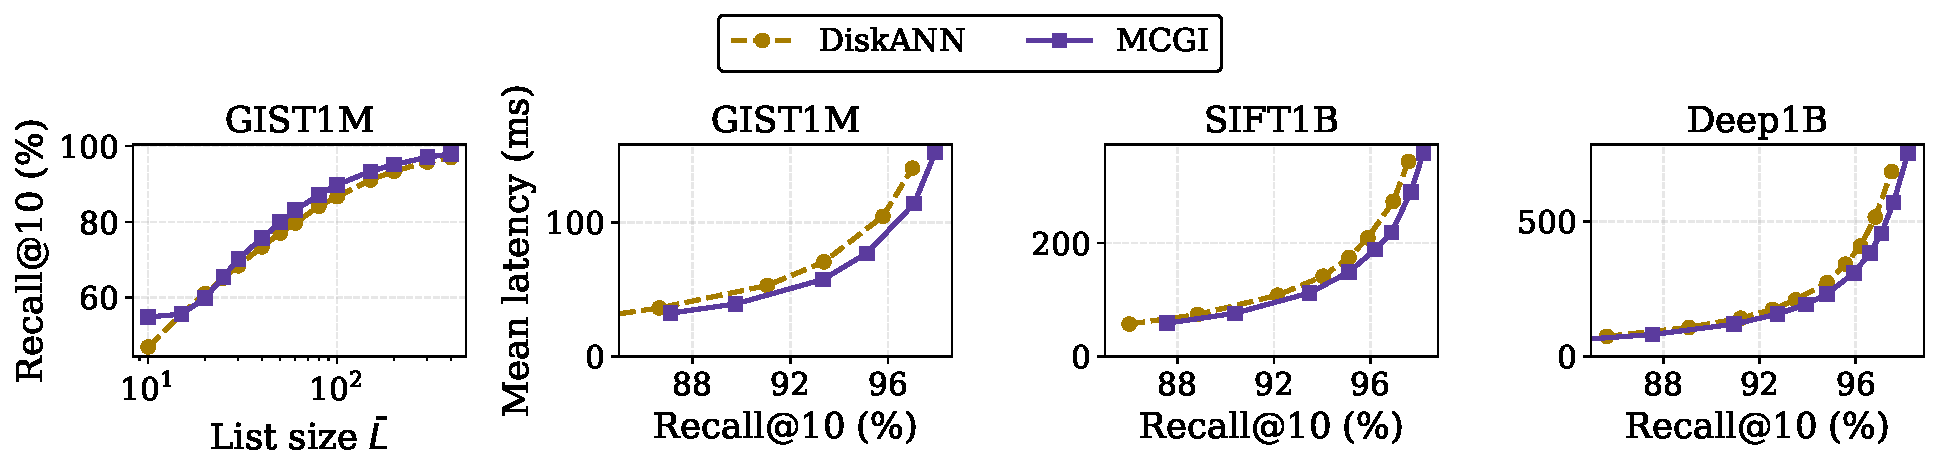
\includegraphics[width=\textwidth]{figures/latency.pdf}
    \caption{Recall against the requested list size, and mean latency against recall.}
    \label{fig:latency}
\end{figure*}

\paragraph{Offline Cost}
Table~\ref{tab:offline_cost} lists the offline cost of each index, where every build runs alone on the platform with 192 threads and the calibration runs alone with 32 search threads. For the million-scale datasets, the table reports a separate rebuild with the same parameters, because the evaluated indexes were built while other jobs shared the machine. The training of the PQ codebooks dominates the build of the million-scale indexes, whereas the graph construction over the shards and their merge dominates at one billion vectors. The only offline step that \ours{} adds is the calibration of Eq.~\eqref{eq:adaptive_list}, which searches the calibration queries once at each list size of a fixed grid and then fits the weights by ridge regression within seconds. The grid has 14 list sizes from 10 to 400 for the million-scale datasets and SIFT1B, and 18 list sizes from 10 to 1{,}000 for Deep1B. Calibration takes about 3 minutes on each million-scale dataset, and 1.6 and 4.8 minutes on SIFT1B and Deep1B, which is at most 1.5\% of the build time of a billion-scale index.

\begin{table}[t]
\centering
\small
\caption{Offline cost in seconds: index build stages and calibration of the query-adaptive search list.}
\label{tab:offline_cost}
\begin{tabular}{lccccc}
\toprule
Dataset & PQ training & Graph & Disk layout & Total build & Calibration \\
\midrule
SIFT1M    & 195   & 6       & 1   & 203       & 174 \\
GloVe-100 & 400   & 15      & 1   & 416       & 168 \\
GIST1M    & 1{,}678 & 82    & 4   & 1{,}764   & 174 \\
SIFT1B    & 2{,}775 & 14{,}117 & 290 & 17{,}225 & 94  \\
Deep1B    & 3{,}373 & 15{,}029 & 836 & 19{,}317 & 289 \\
\bottomrule
\end{tabular}
\end{table}

\subsection{Limitations}
\label{appendix:limitations}

The throughput gains in Section~\ref{sec:experiments} come from the query-adaptive search list, which runs on indexes built with the standard Vamana pruning rule. The construction-time rule of Section~\ref{subsec:mapping} relaxes the pruning test of high-LID nodes; under the degree bound $R$ of a disk-resident index, however, a node fills its neighbor list either way, so that the rule changes which candidate edges a node keeps rather than how many. Consequently, Corollary~\ref{cor:construction_approx} and Proposition~\ref{prop:connectivity} hold without the degree bound, and the evaluation attributes no gain to the construction-time rule.

The query-adaptive list also has costs that its mean throughput does not show. Because hard queries receive lists up to $c$ times longer than $\bar{L}$, the 99.9th-percentile latency at matched recall rises, for example from 119 to 181~ms on GIST1M at 95\% recall, while the mean latency falls. The calibration further needs a few thousand queries from the query distribution together with their exact nearest neighbors, and the fitted weights apply to the index on which they were fitted. Finally, the analysis of Section~\ref{sec:theory} models each beam step as an independent trial whose success probability follows from a uniform local model of the data, so that its bounds describe trends rather than exact recall values.

\subsection{Algorithm Pseudo-Code}
\label{appendix:alg}

Algorithm~\ref{alg:mcgi} outlines the offline construction process of the indexing structure. The procedure is divided into two sequential phases. 
\begin{itemize}
    \item The first phase focuses on geometric calibration by calculating the Local Intrinsic Dimensionality for all vectors in the dataset in parallel. After obtaining the global mean and standard deviation of these estimates, the algorithm assigns a personalized pruning parameter $\alpha_u$ to each node. This parameter is derived using a logistic function that maps the standardized geometric complexity of the local neighborhood into a bounded operational range. 
    \item The second phase handles topology refinement. Starting from a random graph, the algorithm iteratively optimizes the connections. For each node, it executes a greedy search to identify a pool of candidate neighbors. It then evaluates these candidates alongside existing neighbors using a dynamic pruning criterion. A candidate is pruned if a previously accepted neighbor falls within a restricted exclusion region defined by the precomputed $\alpha_u$. Survivors are added to the updated neighbor list until the degree limit is reached.
\end{itemize}

\begin{algorithm}[h!]
   \caption{Manifold-Consistent Graph Indexing (MCGI)}
   \label{alg:mcgi}
\begin{algorithmic}
   \STATE Input: Dataset $X$, Max Degree $R$, Beam Width $L$
   \STATE Output: Optimized Graph $G$

   \STATE
   \STATE // Phase 1: Geometric Calibration
   \STATE $\mathcal{L} \leftarrow \text{ParallelEstimateLID}(X)$
   \STATE $\mu \leftarrow \text{Mean}(\mathcal{L})$
   \STATE $\sigma \leftarrow \text{StdDev}(\mathcal{L})$

   \FOR{each node $u \in V$ in parallel}
       \STATE $z_u \leftarrow (\mathcal{L}[u] - \mu) / \sigma$
       \STATE $\alpha_u \leftarrow \alpha_{\min} + (\alpha_{\max} - \alpha_{\min}) / (1 + \exp(-z_u))$
   \ENDFOR

   \STATE 
   \STATE // Phase 2: Topology Refinement
   \STATE $G \leftarrow \text{RandomGraph}(X, R)$
   
   \FOR{$iter \leftarrow 1$ to $MaxIter$}
       \FOR{each node $u \in G$ in parallel}
           \STATE $\mathcal{C} \leftarrow \text{GreedySearch}(u, G, L)$
           \STATE $\mathcal{N}_{new} \leftarrow \emptyset$
           
           \FOR{$v \in \text{SortByDistance}(\mathcal{C} \cup \mathcal{N}(u))$}
               \STATE $pruned \leftarrow \text{False}$
               \FOR{$n \in \mathcal{N}_{new}$}
                   \IF{$\alpha_u \cdot d(n, v) \le d(u, v)$}
                       \STATE $pruned \leftarrow \text{True}$; break
                   \ENDIF
               \ENDFOR
               \IF{not $pruned$ \AND $|\mathcal{N}_{new}| < R$}
                   \STATE $\mathcal{N}_{new}.\text{add}(v)$
               \ENDIF
           \ENDFOR
           \STATE $\mathcal{N}(u) \leftarrow \mathcal{N}_{new}$
       \ENDFOR
   \ENDFOR
\end{algorithmic}
\end{algorithm}


Algorithm~\ref{alg:online_mcgi} presents an optimized online variant designed to handle massive datasets where exhaustive geometric profiling is computationally prohibitive. 
\begin{itemize}
    \item It begins with a fast approximation phase that samples a small subset of the data. By evaluating this subset, the algorithm quickly bootstraps the global mean and standard deviation of the underlying probability distribution. This step provides a coarse but efficient estimate of the overall geometric complexity, enabling the algorithm to initialize the pruning parameters without incurring the cost of a full dataset pass.
    \item The second phase merges the geometric estimation directly into the iterative topology refinement loop. Instead of computing all complexities beforehand, the algorithm dynamically estimates the node specific dimensionality on the fly using the candidate set discovered during the greedy search step. This real time estimate is immediately used to calculate the specific pruning parameter $\alpha_u$. The algorithm then applies this dynamic parameter to the pruning criterion, determining which edges to preserve and which to discard. This approach ensures the graph connectivity adapts to the manifold geometry progressively as the quality of the candidate neighbors improves with each iteration.
\end{itemize}

\begin{algorithm}[h!]
   \caption{Online Manifold-Consistent Graph Indexing}
   \label{alg:online_mcgi}
\begin{algorithmic}
   \STATE Input: Dataset $X$, Max Degree $R$, Beam Width $L$, Sample Rate $S$
   \STATE Output: Optimized Graph $G$

   \STATE
   \STATE // Phase 1: Bootstrap Statistics (Fast Approximation)
   \STATE $X_{sample} \leftarrow \text{RandomSample}(X, S)$
   \STATE $\mathcal{L}_{sample} \leftarrow \text{EstimateLID}(X_{sample})$ \COMMENT{Compute LID on subset}
   \STATE $\mu \leftarrow \text{Mean}(\mathcal{L}_{sample})$, $\sigma \leftarrow \text{StdDev}(\mathcal{L}_{sample})$

   \STATE 
   \STATE // Phase 2: Online Topology Refinement
   \STATE $G \leftarrow \text{RandomGraph}(X, R)$
   
   \FOR{$iter \leftarrow 1$ to $MaxIter$}
       \FOR{each node $u \in G$ in parallel}
           \STATE $\mathcal{C} \leftarrow \text{GreedySearch}(u, G, L)$
           
           \STATE // Online LID Estimation \& Parameter Adaptation
           \STATE $\hat{\ell}_u \leftarrow \text{ComputeLID}(u, \mathcal{C})$ \COMMENT{Estimate from neighbors}
           \STATE $z_u \leftarrow (\hat{\ell}_u - \mu) / \sigma$
           \STATE $\alpha_u \leftarrow \alpha_{\min} + (\alpha_{\max} - \alpha_{\min}) / (1 + \exp(-z_u))$

           \STATE $\mathcal{N}_{new} \leftarrow \emptyset$
           
           \FOR{$v \in \text{SortByDistance}(\mathcal{C} \cup \mathcal{N}(u))$}
               \STATE $pruned \leftarrow \text{False}$
               \FOR{$n \in \mathcal{N}_{new}$}
                   \STATE // Pruning with dynamic $\alpha_u$
                   \IF{$\alpha_u \cdot d(n, v) \le d(u, v)$}
                       \STATE $pruned \leftarrow \text{True}$; break
                   \ENDIF
               \ENDFOR
               \IF{not $pruned$ \AND $|\mathcal{N}_{new}| < R$}
                   \STATE $\mathcal{N}_{new}.\text{add}(v)$
               \ENDIF
           \ENDFOR
           \STATE $\mathcal{N}(u) \leftarrow \mathcal{N}_{new}$
       \ENDFOR
   \ENDFOR
\end{algorithmic}
\end{algorithm}

\end{document}